\documentclass[twoside]{book}

% Packages required by doxygen
\usepackage{calc}
\usepackage{doxygen}
\usepackage{graphicx}
\usepackage[utf8]{inputenc}
\usepackage{makeidx}
\usepackage{multicol}
\usepackage{multirow}
\usepackage{fixltx2e}
\PassOptionsToPackage{warn}{textcomp}
\usepackage{textcomp}
\usepackage[nointegrals]{wasysym}
\usepackage[table]{xcolor}

% Font selection
\usepackage[T1]{fontenc}
\usepackage{mathptmx}
\usepackage[scaled=.90]{helvet}
\usepackage{courier}
\usepackage{amssymb}
\usepackage{sectsty}
\renewcommand{\familydefault}{\sfdefault}
\allsectionsfont{%
  \fontseries{bc}\selectfont%
  \color{darkgray}%
}
\renewcommand{\DoxyLabelFont}{%
  \fontseries{bc}\selectfont%
  \color{darkgray}%
}
\newcommand{\+}{\discretionary{\mbox{\scriptsize$\hookleftarrow$}}{}{}}

% Page & text layout
\usepackage{geometry}
\geometry{%
  a4paper,%
  top=2.5cm,%
  bottom=2.5cm,%
  left=2.5cm,%
  right=2.5cm%
}
\tolerance=750
\hfuzz=15pt
\hbadness=750
\setlength{\emergencystretch}{15pt}
\setlength{\parindent}{0cm}
\setlength{\parskip}{0.2cm}
\makeatletter
\renewcommand{\paragraph}{%
  \@startsection{paragraph}{4}{0ex}{-1.0ex}{1.0ex}{%
    \normalfont\normalsize\bfseries\SS@parafont%
  }%
}
\renewcommand{\subparagraph}{%
  \@startsection{subparagraph}{5}{0ex}{-1.0ex}{1.0ex}{%
    \normalfont\normalsize\bfseries\SS@subparafont%
  }%
}
\makeatother

% Headers & footers
\usepackage{fancyhdr}
\pagestyle{fancyplain}
\fancyhead[LE]{\fancyplain{}{\bfseries\thepage}}
\fancyhead[CE]{\fancyplain{}{}}
\fancyhead[RE]{\fancyplain{}{\bfseries\leftmark}}
\fancyhead[LO]{\fancyplain{}{\bfseries\rightmark}}
\fancyhead[CO]{\fancyplain{}{}}
\fancyhead[RO]{\fancyplain{}{\bfseries\thepage}}
\fancyfoot[LE]{\fancyplain{}{}}
\fancyfoot[CE]{\fancyplain{}{}}
\fancyfoot[RE]{\fancyplain{}{\bfseries\scriptsize Generated on Sat Jul 12 2014 12\+:17\+:19 for Cmd\+Messenger by Doxygen }}
\fancyfoot[LO]{\fancyplain{}{\bfseries\scriptsize Generated on Sat Jul 12 2014 12\+:17\+:19 for Cmd\+Messenger by Doxygen }}
\fancyfoot[CO]{\fancyplain{}{}}
\fancyfoot[RO]{\fancyplain{}{}}
\renewcommand{\footrulewidth}{0.4pt}
\renewcommand{\chaptermark}[1]{%
  \markboth{#1}{}%
}
\renewcommand{\sectionmark}[1]{%
  \markright{\thesection\ #1}%
}

% Indices & bibliography
\usepackage{natbib}
\usepackage[titles]{tocloft}
\setcounter{tocdepth}{3}
\setcounter{secnumdepth}{5}
\makeindex

% Hyperlinks (required, but should be loaded last)
\usepackage{ifpdf}
\ifpdf
  \usepackage[pdftex,pagebackref=true]{hyperref}
\else
  \usepackage[ps2pdf,pagebackref=true]{hyperref}
\fi
\hypersetup{%
  colorlinks=true,%
  linkcolor=blue,%
  citecolor=blue,%
  unicode%
}

% Custom commands
\newcommand{\clearemptydoublepage}{%
  \newpage{\pagestyle{empty}\cleardoublepage}%
}


%===== C O N T E N T S =====

\begin{document}

% Titlepage & ToC
\hypersetup{pageanchor=false,
             bookmarks=true,
             bookmarksnumbered=true,
             pdfencoding=unicode
            }
\pagenumbering{roman}
\begin{titlepage}
\vspace*{7cm}
\begin{center}%
{\Large Cmd\+Messenger }\\
\vspace*{1cm}
{\large Generated by Doxygen 1.8.7}\\
\vspace*{0.5cm}
{\small Sat Jul 12 2014 12:17:19}\\
\end{center}
\end{titlepage}
\clearemptydoublepage
\tableofcontents
\clearemptydoublepage
\pagenumbering{arabic}
\hypersetup{pageanchor=true}

%--- Begin generated contents ---
\chapter{Cmd\+Messenger C++ Implementation}
\label{index}\hypertarget{index}{}\begin{DoxyAuthor}{Author}
Rodrigues Filho \href{mailto:edno-moura@mail.com}{\tt edno-\/moura@mail.\+com}
\end{DoxyAuthor}
\hypertarget{index_what_is}{}\section{What is Cmd\+Messenger?}\label{index_what_is}
The Cmd\+Messenger is a messaging library for the Arduino platform. To use the Cmd\+Messenger, a list of command identifiers is defined and then, callbacks are attached for the received messages. The message format is as it follows\+: 
\begin{DoxyPre}
  cmdID,arg1,arg2,...,argn;
\end{DoxyPre}
\hypertarget{index_this_project}{}\section{What is this project all about?}\label{index_this_project}
This is simply an implementation of such messaging protocol for the pc side, built in a cross-\/platform C++. It uses the Serial Library for its communication, this library provides total control over Timeouts and it is cross-\/platform. The official project of the Cmd\+Messenger provides a full C\# implementation that runs in both Mono and Visual Studio.\hypertarget{index_getting_started}{}\section{Getting Started}\label{index_getting_started}
Take a look at the main class documentation \hyperlink{classcmd_1_1_cmd_messenger}{cmd\+::\+Cmd\+Messenger} and the command classes \hyperlink{classcmd_1_1_cmd_received}{cmd\+::\+Cmd\+Received} \hyperlink{classcmd_1_1_cmd_send}{cmd\+::\+Cmd\+Send}

Take a look at this simple example \hyperlink{led_8cpp}{led.\+cpp}\hypertarget{index_features}{}\section{Features}\label{index_features}

\begin{DoxyItemize}
\item Total control over Timeouts trough the Serial Library project.
\item Send and receive ascii commands.
\item Clean A\+P\+I with overloaded operators.
\item Set methods or global functions as callbacks.
\end{DoxyItemize}\hypertarget{index_problems}{}\section{Problems}\label{index_problems}

\begin{DoxyItemize}
\item Does not send or receive binary data.
\item Parsers safety and efficiency needs to be improved.
\item It's written in cross-\/platform C++, but the project lacks support for other platforms rather than linux.
\end{DoxyItemize}\hypertarget{index_install}{}\section{Installation}\label{index_install}
\begin{DoxyRefDesc}{Todo}
\item[\hyperlink{todo__todo000001}{Todo}]Write the install section 

Remember to find a way to ship all dependecies in one package \end{DoxyRefDesc}

\chapter{Todo List}
\label{todo}
\hypertarget{todo}{}

\begin{DoxyRefList}
\item[\label{todo__todo000003}%
\hypertarget{todo__todo000003}{}%
Namespace \hyperlink{namespacecmd}{cmd} ]Exceptions for parsing erros and empty queues 

Improve the parser to implement escaping (check how this was done in the arduino implementation).  
\item[\label{todo__todo000001}%
\hypertarget{todo__todo000001}{}%
page \hyperlink{index}{Cmd\+Messenger C++ Implementation} ]write the getting started section 

Remember to find a way to ship all dependecies in one package 

Throw exceptions

Write the install section  
\item[\label{todo__todo000004}%
\hypertarget{todo__todo000004}{}%
File \hyperlink{_cmd_messenger_8cpp}{Cmd\+Messenger.cpp} ]this license
\end{DoxyRefList}
\chapter{Namespace Index}
\section{Namespace List}
Here is a list of all namespaces with brief descriptions\+:\begin{DoxyCompactList}
\item\contentsline{section}{\hyperlink{namespacecmd}{cmd} }{\pageref{namespacecmd}}{}
\end{DoxyCompactList}

\chapter{Hierarchical Index}
\section{Class Hierarchy}
This inheritance list is sorted roughly, but not completely, alphabetically\+:\begin{DoxyCompactList}
\item \contentsline{section}{Cmd\+Base}{\pageref{class_cmd_base}}{}
\begin{DoxyCompactList}
\item \contentsline{section}{cmd\+:\+:Cmd\+Received}{\pageref{classcmd_1_1_cmd_received}}{}
\item \contentsline{section}{cmd\+:\+:Cmd\+Send}{\pageref{classcmd_1_1_cmd_send}}{}
\end{DoxyCompactList}
\item \contentsline{section}{Cmd\+End}{\pageref{class_cmd_end}}{}
\item \contentsline{section}{cmd\+:\+:Cmd\+Messenger}{\pageref{classcmd_1_1_cmd_messenger}}{}
\item \contentsline{section}{Transport\+Layer}{\pageref{class_transport_layer}}{}
\end{DoxyCompactList}

\chapter{Data Structure Index}
\section{Data Structures}
Here are the data structures with brief descriptions\+:\begin{DoxyCompactList}
\item\contentsline{section}{\hyperlink{classcallback}{callback} }{\pageref{classcallback}}{}
\item\contentsline{section}{\hyperlink{class_cmd_base}{Cmd\+Base} }{\pageref{class_cmd_base}}{}
\item\contentsline{section}{\hyperlink{class_cmd_end}{Cmd\+End} }{\pageref{class_cmd_end}}{}
\item\contentsline{section}{\hyperlink{classcmd_1_1_cmd_messenger}{cmd\+::\+Cmd\+Messenger} }{\pageref{classcmd_1_1_cmd_messenger}}{}
\item\contentsline{section}{\hyperlink{classcmd_1_1_cmd_received}{cmd\+::\+Cmd\+Received} }{\pageref{classcmd_1_1_cmd_received}}{}
\item\contentsline{section}{\hyperlink{classcmd_1_1_cmd_send}{cmd\+::\+Cmd\+Send} }{\pageref{classcmd_1_1_cmd_send}}{}
\end{DoxyCompactList}

\chapter{File Index}
\section{File List}
Here is a list of all files with brief descriptions\+:\begin{DoxyCompactList}
\item\contentsline{section}{/home/edno/projetos/cmd\+Messenger-\/cpp/include/\hyperlink{_cmd_base_8h}{Cmd\+Base.\+h} }{\pageref{_cmd_base_8h}}{}
\item\contentsline{section}{/home/edno/projetos/cmd\+Messenger-\/cpp/include/\hyperlink{_cmd_messenger_8h}{Cmd\+Messenger.\+h} }{\pageref{_cmd_messenger_8h}}{}
\item\contentsline{section}{/home/edno/projetos/cmd\+Messenger-\/cpp/include/\hyperlink{_cmd_received_8h}{Cmd\+Received.\+h} }{\pageref{_cmd_received_8h}}{}
\item\contentsline{section}{/home/edno/projetos/cmd\+Messenger-\/cpp/include/\hyperlink{_cmd_send_8h}{Cmd\+Send.\+h} }{\pageref{_cmd_send_8h}}{}
\item\contentsline{section}{/home/edno/projetos/cmd\+Messenger-\/cpp/include/\hyperlink{_serial_transport_8h}{Serial\+Transport.\+h} }{\pageref{_serial_transport_8h}}{}
\item\contentsline{section}{/home/edno/projetos/cmd\+Messenger-\/cpp/include/\hyperlink{_transport_layer_8h}{Transport\+Layer.\+h} }{\pageref{_transport_layer_8h}}{}
\item\contentsline{section}{/home/edno/projetos/cmd\+Messenger-\/cpp/src/\hyperlink{_cmd_base_8cpp}{Cmd\+Base.\+cpp} }{\pageref{_cmd_base_8cpp}}{}
\item\contentsline{section}{/home/edno/projetos/cmd\+Messenger-\/cpp/src/\hyperlink{_cmd_messenger_8cpp}{Cmd\+Messenger.\+cpp} }{\pageref{_cmd_messenger_8cpp}}{}
\item\contentsline{section}{/home/edno/projetos/cmd\+Messenger-\/cpp/src/\hyperlink{_cmd_received_8cpp}{Cmd\+Received.\+cpp} }{\pageref{_cmd_received_8cpp}}{}
\item\contentsline{section}{/home/edno/projetos/cmd\+Messenger-\/cpp/src/\hyperlink{_cmd_send_8cpp}{Cmd\+Send.\+cpp} }{\pageref{_cmd_send_8cpp}}{}
\item\contentsline{section}{/home/edno/projetos/cmd\+Messenger-\/cpp/src/examples/\hyperlink{led_8cpp}{led.\+cpp} }{\pageref{led_8cpp}}{}
\item\contentsline{section}{/home/edno/projetos/cmd\+Messenger-\/cpp/src/examples/\hyperlink{sensor_8cpp}{sensor.\+cpp} }{\pageref{sensor_8cpp}}{}
\end{DoxyCompactList}

\chapter{Namespace Documentation}
\hypertarget{namespacecmd}{\section{cmd Namespace Reference}
\label{namespacecmd}\index{cmd@{cmd}}
}
\subsection*{Data Structures}
\begin{DoxyCompactItemize}
\item 
class \hyperlink{classcmd_1_1_cmd_messenger}{Cmd\+Messenger}
\item 
class \hyperlink{classcmd_1_1_cmd_received}{Cmd\+Received}
\item 
class \hyperlink{classcmd_1_1_cmd_send}{Cmd\+Send}
\end{DoxyCompactItemize}
\subsection*{Typedefs}
\begin{DoxyCompactItemize}
\item 
typedef \hyperlink{classcmd_1_1_cmd_send}{Cmd\+Send} \hyperlink{namespacecmd_af9b58ca395c80edd1335e21d1b9f4c99}{Cmd}
\item 
typedef void($\ast$ \hyperlink{namespacecmd_a20b40ecd3ba46130eef6c125f70c4121}{Call\+Back} )(\hyperlink{classcmd_1_1_cmd_received}{Cmd\+Received} \&)
\end{DoxyCompactItemize}


\subsection{Detailed Description}
\begin{DoxyRefDesc}{Todo}
\item[\hyperlink{todo__todo000003}{Todo}]Exceptions for parsing erros and empty queues 

Improve the parser to implement escaping (check how this was done in the arduino implementation). \end{DoxyRefDesc}


\subsection{Typedef Documentation}
\hypertarget{namespacecmd_a20b40ecd3ba46130eef6c125f70c4121}{\index{cmd@{cmd}!Call\+Back@{Call\+Back}}
\index{Call\+Back@{Call\+Back}!cmd@{cmd}}
\subsubsection[{Call\+Back}]{\setlength{\rightskip}{0pt plus 5cm}typedef void($\ast$ cmd\+::\+Call\+Back)({\bf Cmd\+Received} \&)}}\label{namespacecmd_a20b40ecd3ba46130eef6c125f70c4121}


Definition at line 90 of file Cmd\+Messenger.\+h.

\hypertarget{namespacecmd_af9b58ca395c80edd1335e21d1b9f4c99}{\index{cmd@{cmd}!Cmd@{Cmd}}
\index{Cmd@{Cmd}!cmd@{cmd}}
\subsubsection[{Cmd}]{\setlength{\rightskip}{0pt plus 5cm}typedef {\bf Cmd\+Send} {\bf cmd\+::\+Cmd}}}\label{namespacecmd_af9b58ca395c80edd1335e21d1b9f4c99}


Definition at line 89 of file Cmd\+Messenger.\+h.


\chapter{Data Structure Documentation}
\hypertarget{classcallback}{\section{callback Class Reference}
\label{classcallback}\index{callback@{callback}}
}
\subsection*{Public Member Functions}
\begin{DoxyCompactItemize}
\item 
\hyperlink{classcallback_a0d8f5143653fb6d1d6e46603e03a7525}{callback} ()
\item 
\hyperlink{classcallback_a630ccfaeea6fc3f676e38e8a75dc6155}{$\sim$callback} ()
\end{DoxyCompactItemize}
\subsection*{Static Public Member Functions}
\begin{DoxyCompactItemize}
\item 
static void \hyperlink{classcallback_a35a5ce520719e5c4f49f59ebe9406db9}{method} (\hyperlink{classcmd_1_1_cmd_received}{cmd\+::\+Cmd\+Received} \&command)
\end{DoxyCompactItemize}


\subsection{Detailed Description}


Definition at line 13 of file led.\+cpp.



\subsection{Constructor \& Destructor Documentation}
\hypertarget{classcallback_a0d8f5143653fb6d1d6e46603e03a7525}{\index{callback@{callback}!callback@{callback}}
\index{callback@{callback}!callback@{callback}}
\subsubsection[{callback}]{\setlength{\rightskip}{0pt plus 5cm}callback\+::callback (
\begin{DoxyParamCaption}
{}
\end{DoxyParamCaption}
)\hspace{0.3cm}{\ttfamily [inline]}}}\label{classcallback_a0d8f5143653fb6d1d6e46603e03a7525}


Definition at line 17 of file led.\+cpp.

\hypertarget{classcallback_a630ccfaeea6fc3f676e38e8a75dc6155}{\index{callback@{callback}!````~callback@{$\sim$callback}}
\index{````~callback@{$\sim$callback}!callback@{callback}}
\subsubsection[{$\sim$callback}]{\setlength{\rightskip}{0pt plus 5cm}callback\+::$\sim$callback (
\begin{DoxyParamCaption}
{}
\end{DoxyParamCaption}
)\hspace{0.3cm}{\ttfamily [inline]}}}\label{classcallback_a630ccfaeea6fc3f676e38e8a75dc6155}


Definition at line 18 of file led.\+cpp.



\subsection{Member Function Documentation}
\hypertarget{classcallback_a35a5ce520719e5c4f49f59ebe9406db9}{\index{callback@{callback}!method@{method}}
\index{method@{method}!callback@{callback}}
\subsubsection[{method}]{\setlength{\rightskip}{0pt plus 5cm}static void callback\+::method (
\begin{DoxyParamCaption}
\item[{{\bf cmd\+::\+Cmd\+Received} \&}]{command}
\end{DoxyParamCaption}
)\hspace{0.3cm}{\ttfamily [inline]}, {\ttfamily [static]}}}\label{classcallback_a35a5ce520719e5c4f49f59ebe9406db9}


Definition at line 20 of file led.\+cpp.



The documentation for this class was generated from the following file\+:\begin{DoxyCompactItemize}
\item 
/home/edno/projetos/robot/cmd\+Messenger-\/cpp/src/examples/\hyperlink{led_8cpp}{led.\+cpp}\end{DoxyCompactItemize}

\hypertarget{class_cmd_base}{\section{Cmd\+Base Class Reference}
\label{class_cmd_base}\index{Cmd\+Base@{Cmd\+Base}}
}


{\ttfamily \#include $<$Cmd\+Base.\+h$>$}

Inheritance diagram for Cmd\+Base\+:\begin{figure}[H]
\begin{center}
\leavevmode
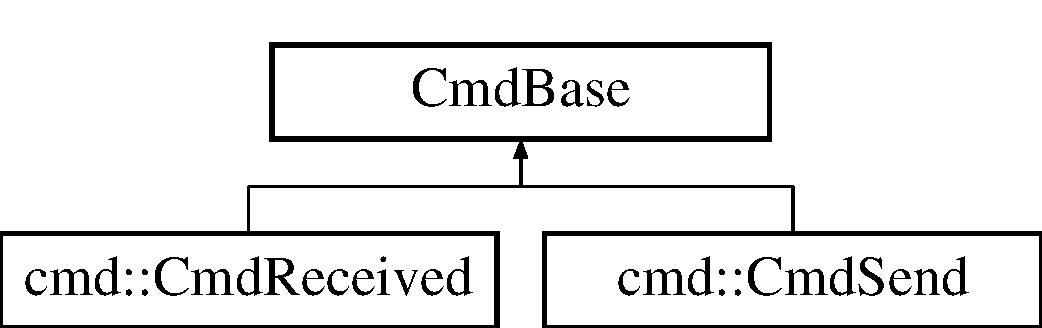
\includegraphics[height=2.000000cm]{class_cmd_base}
\end{center}
\end{figure}
\subsection*{Public Member Functions}
\begin{DoxyCompactItemize}
\item 
\hyperlink{class_cmd_base_a33bf0141fa7a6f77ccfe84d3ce144ca9}{Cmd\+Base} (int id=0)
\item 
virtual \hyperlink{class_cmd_base_a79d89d75709596e426ef412883ba4c91}{$\sim$\+Cmd\+Base} ()
\item 
void \hyperlink{class_cmd_base_ac83aced054abdb8e39b358bf109378d6}{set\+Id} (int id)
\item 
int \hyperlink{class_cmd_base_afcf8a525095025adb2ebf7304511b006}{get\+Id} () const 
\end{DoxyCompactItemize}


\subsection{Detailed Description}
Base class for commands (Send and Received commands). 

Definition at line 49 of file Cmd\+Base.\+h.



\subsection{Constructor \& Destructor Documentation}
\hypertarget{class_cmd_base_a33bf0141fa7a6f77ccfe84d3ce144ca9}{\index{Cmd\+Base@{Cmd\+Base}!Cmd\+Base@{Cmd\+Base}}
\index{Cmd\+Base@{Cmd\+Base}!Cmd\+Base@{Cmd\+Base}}
\subsubsection[{Cmd\+Base}]{\setlength{\rightskip}{0pt plus 5cm}Cmd\+Base\+::\+Cmd\+Base (
\begin{DoxyParamCaption}
\item[{int}]{id = {\ttfamily 0}}
\end{DoxyParamCaption}
)}}\label{class_cmd_base_a33bf0141fa7a6f77ccfe84d3ce144ca9}


Definition at line 3 of file Cmd\+Base.\+cpp.

\hypertarget{class_cmd_base_a79d89d75709596e426ef412883ba4c91}{\index{Cmd\+Base@{Cmd\+Base}!````~Cmd\+Base@{$\sim$\+Cmd\+Base}}
\index{````~Cmd\+Base@{$\sim$\+Cmd\+Base}!Cmd\+Base@{Cmd\+Base}}
\subsubsection[{$\sim$\+Cmd\+Base}]{\setlength{\rightskip}{0pt plus 5cm}Cmd\+Base\+::$\sim$\+Cmd\+Base (
\begin{DoxyParamCaption}
{}
\end{DoxyParamCaption}
)\hspace{0.3cm}{\ttfamily [virtual]}}}\label{class_cmd_base_a79d89d75709596e426ef412883ba4c91}


Definition at line 8 of file Cmd\+Base.\+cpp.



\subsection{Member Function Documentation}
\hypertarget{class_cmd_base_afcf8a525095025adb2ebf7304511b006}{\index{Cmd\+Base@{Cmd\+Base}!get\+Id@{get\+Id}}
\index{get\+Id@{get\+Id}!Cmd\+Base@{Cmd\+Base}}
\subsubsection[{get\+Id}]{\setlength{\rightskip}{0pt plus 5cm}int Cmd\+Base\+::get\+Id (
\begin{DoxyParamCaption}
{}
\end{DoxyParamCaption}
) const}}\label{class_cmd_base_afcf8a525095025adb2ebf7304511b006}


Definition at line 17 of file Cmd\+Base.\+cpp.

\hypertarget{class_cmd_base_ac83aced054abdb8e39b358bf109378d6}{\index{Cmd\+Base@{Cmd\+Base}!set\+Id@{set\+Id}}
\index{set\+Id@{set\+Id}!Cmd\+Base@{Cmd\+Base}}
\subsubsection[{set\+Id}]{\setlength{\rightskip}{0pt plus 5cm}void Cmd\+Base\+::set\+Id (
\begin{DoxyParamCaption}
\item[{int}]{id}
\end{DoxyParamCaption}
)}}\label{class_cmd_base_ac83aced054abdb8e39b358bf109378d6}


Definition at line 12 of file Cmd\+Base.\+cpp.



The documentation for this class was generated from the following files\+:\begin{DoxyCompactItemize}
\item 
/home/edno/projetos/cmd\+Messenger-\/cpp/include/\hyperlink{_cmd_base_8h}{Cmd\+Base.\+h}\item 
/home/edno/projetos/cmd\+Messenger-\/cpp/src/\hyperlink{_cmd_base_8cpp}{Cmd\+Base.\+cpp}\end{DoxyCompactItemize}

\hypertarget{class_cmd_end}{\section{Cmd\+End Class Reference}
\label{class_cmd_end}\index{Cmd\+End@{Cmd\+End}}
}


{\ttfamily \#include $<$Cmd\+Base.\+h$>$}



\subsection{Detailed Description}
An empyt class that indicates the end of a command 

Definition at line 44 of file Cmd\+Base.\+h.



The documentation for this class was generated from the following file\+:\begin{DoxyCompactItemize}
\item 
/home/edno/projetos/cmd\+Messenger-\/cpp/include/\hyperlink{_cmd_base_8h}{Cmd\+Base.\+h}\end{DoxyCompactItemize}

\hypertarget{classcmd_1_1_cmd_messenger}{\section{cmd\+:\+:Cmd\+Messenger Class Reference}
\label{classcmd_1_1_cmd_messenger}\index{cmd\+::\+Cmd\+Messenger@{cmd\+::\+Cmd\+Messenger}}
}


{\ttfamily \#include $<$Cmd\+Messenger.\+h$>$}

\subsection*{Public Member Functions}
\begin{DoxyCompactItemize}
\item 
\hyperlink{classcmd_1_1_cmd_messenger_aba80ae7cc283a24b7afa08c18f89af0f}{Cmd\+Messenger} (const std\+::string \&port=\char`\"{}\char`\"{}, uint32\+\_\+t baudrate=9600, const char field\+\_\+separator= ',', const char cmd\+\_\+separator= ';', const char esc\+\_\+character= '/', Timeout timeout=Timeout(), bytesize\+\_\+t bytesize=eightbits, parity\+\_\+t parity=parity\+\_\+none, stopbits\+\_\+t stopbits=stopbits\+\_\+one, flowcontrol\+\_\+t flowcontrol=flowcontrol\+\_\+none)
\item 
virtual \hyperlink{classcmd_1_1_cmd_messenger_aa92b483212121faffeb02b7a63450ad0}{$\sim$\+Cmd\+Messenger} ()
\item 
void \hyperlink{classcmd_1_1_cmd_messenger_adb4617437e81ccb39b1d314b83db8f6c}{open} ()
\item 
bool \hyperlink{classcmd_1_1_cmd_messenger_a38dab46f4b3c0c56e8dad6e91b9500c8}{is\+Open} () const 
\item 
void \hyperlink{classcmd_1_1_cmd_messenger_a3a08819cae57dd6c9f7515ebae923696}{close} ()
\item 
void \hyperlink{classcmd_1_1_cmd_messenger_a92df6db7de8ce3d685d4da21b7c76d77}{attach} (\hyperlink{namespacecmd_a20b40ecd3ba46130eef6c125f70c4121}{Call\+Back} callback)
\item 
{\footnotesize template$<$typename T $>$ }\\void \hyperlink{classcmd_1_1_cmd_messenger_a5af33d07f7074623701f822a6cb7ee81}{attach} (void(T\+::$\ast$callback\+\_\+method)(\hyperlink{classcmd_1_1_cmd_received}{Cmd\+Received} \&), T \&object\+\_\+ref)
\item 
void \hyperlink{classcmd_1_1_cmd_messenger_abbc2aa2a6bc95960215eeaa88c4533a4}{attach} (int cmd\+\_\+id, \hyperlink{namespacecmd_a20b40ecd3ba46130eef6c125f70c4121}{Call\+Back} callback)
\item 
{\footnotesize template$<$typename T $>$ }\\void \hyperlink{classcmd_1_1_cmd_messenger_a8f50f00a66e6d40ed5ee2234b424e9a9}{attach} (int cmd\+\_\+id, void(T\+::$\ast$callback\+\_\+method)(\hyperlink{classcmd_1_1_cmd_received}{Cmd\+Received} \&), T \&object\+\_\+ref)
\item 
bool \hyperlink{classcmd_1_1_cmd_messenger_a5ea6815a9c6dad49350396839527e25d}{send} (const \hyperlink{namespacecmd_af9b58ca395c80edd1335e21d1b9f4c99}{Cmd} \&command, bool ack=false, int ack\+\_\+id=0, int simple\+\_\+timeout=-\/1)
\item 
bool \hyperlink{classcmd_1_1_cmd_messenger_a40c20df2763d3af8e59a7c135a82e121}{wait\+Cmd} (int cmd\+\_\+id, int simple\+\_\+timeout=-\/1)
\item 
void \hyperlink{classcmd_1_1_cmd_messenger_a3257cf2b159a2b3d8754b701865c743d}{feed\+In\+Serial\+Data} ()
\item 
void \hyperlink{classcmd_1_1_cmd_messenger_af83fbed5873f5e517a0432438dd7c873}{set\+Field\+Sep} (const char field\+\_\+separator)
\item 
char \hyperlink{classcmd_1_1_cmd_messenger_a84895ecc82e2302891b119887944a308}{get\+Field\+Sep} () const 
\item 
void \hyperlink{classcmd_1_1_cmd_messenger_afebb6b63ae64c661b680597ef29bc879}{set\+Cmd\+Sep} (const char cmd\+\_\+separator)
\item 
char \hyperlink{classcmd_1_1_cmd_messenger_acfa9dda9411bc8943973abd5f5f6156f}{get\+Cmd\+Sep} () const 
\item 
void \hyperlink{classcmd_1_1_cmd_messenger_ada69819065773ffc3c4923517321d6e5}{set\+Esc\+Char} (const char esc\+\_\+character)
\item 
char \hyperlink{classcmd_1_1_cmd_messenger_adf36d1a1b153793d9bf33f14b26167a5}{get\+Esc\+Char} () const 
\item 
void \hyperlink{classcmd_1_1_cmd_messenger_ab95dce49fc8845498c71bae25987a923}{set\+Port} (const std\+::string \&port)
\item 
std\+::string \hyperlink{classcmd_1_1_cmd_messenger_ab2ebaaabdfeb83decbc868b556a1ea0b}{get\+Port} () const 
\item 
void \hyperlink{classcmd_1_1_cmd_messenger_a0ccea65cba7a807bdf4c476f8db9289a}{set\+Timeout} (Timeout \&timeout)
\item 
void \hyperlink{classcmd_1_1_cmd_messenger_a0d628c1961f8d2b96fa7081961f6a0c1}{set\+Timeout} (uint32\+\_\+t inter\+\_\+byte\+\_\+timeout, uint32\+\_\+t read\+\_\+timeout\+\_\+constant, uint32\+\_\+t read\+\_\+timeout\+\_\+multiplier, uint32\+\_\+t write\+\_\+timeout\+\_\+constant, uint32\+\_\+t write\+\_\+timeout\+\_\+multiplier)
\item 
Timeout \hyperlink{classcmd_1_1_cmd_messenger_a6b8a4f763475a9e4fbef2237f1050849}{get\+Timeout} () const 
\item 
void \hyperlink{classcmd_1_1_cmd_messenger_a0fc1bac4fc0d3494893113ade503099b}{set\+Baud\+Rate} (uint32\+\_\+t baudrate)
\item 
uint32\+\_\+t \hyperlink{classcmd_1_1_cmd_messenger_a14c580579b5311ff78cce8de34fe63b2}{get\+Baudrate} () const 
\item 
void \hyperlink{classcmd_1_1_cmd_messenger_ae05db8b37c1b2ee9be47ea3a3bf045bd}{set\+Byte\+Size} (bytesize\+\_\+t bytesize)
\item 
bytesize\+\_\+t \hyperlink{classcmd_1_1_cmd_messenger_a8ccc24a1f621afd1e114696ed9b8b261}{get\+Byte\+Size} () const 
\item 
void \hyperlink{classcmd_1_1_cmd_messenger_ae0bbc0b786fadff310f31c84644b56c5}{set\+Parity} (parity\+\_\+t parity)
\item 
parity\+\_\+t \hyperlink{classcmd_1_1_cmd_messenger_ad487f6fd40a2bffc69fab5334d96ab52}{get\+Parity} () const 
\item 
void \hyperlink{classcmd_1_1_cmd_messenger_a06eaedc3c9e7b0b3cda7b139ee61f5bb}{set\+Stop\+Bits} (stopbits\+\_\+t stopbits)
\item 
stopbits\+\_\+t \hyperlink{classcmd_1_1_cmd_messenger_a2dd6e45584ed65ff1f744e46198e7755}{get\+Stop\+Bits} () const 
\item 
void \hyperlink{classcmd_1_1_cmd_messenger_a5271d79b0f4ae95bea5897b214fbbd4c}{set\+Flow\+Control} (flowcontrol\+\_\+t flowcontrol)
\item 
flowcontrol\+\_\+t \hyperlink{classcmd_1_1_cmd_messenger_a11e2bea7282a912fd05644b403b55503}{get\+Flow\+Control} () const 
\end{DoxyCompactItemize}


\subsection{Detailed Description}


Definition at line 95 of file Cmd\+Messenger.\+h.



\subsection{Constructor \& Destructor Documentation}
\hypertarget{classcmd_1_1_cmd_messenger_aba80ae7cc283a24b7afa08c18f89af0f}{\index{cmd\+::\+Cmd\+Messenger@{cmd\+::\+Cmd\+Messenger}!Cmd\+Messenger@{Cmd\+Messenger}}
\index{Cmd\+Messenger@{Cmd\+Messenger}!cmd\+::\+Cmd\+Messenger@{cmd\+::\+Cmd\+Messenger}}
\subsubsection[{Cmd\+Messenger}]{\setlength{\rightskip}{0pt plus 5cm}Cmd\+Messenger\+::\+Cmd\+Messenger (
\begin{DoxyParamCaption}
\item[{const std\+::string \&}]{port = {\ttfamily \char`\"{}\char`\"{}}, }
\item[{uint32\+\_\+t}]{baudrate = {\ttfamily 9600}, }
\item[{const char}]{field\+\_\+separator = {\ttfamily ','}, }
\item[{const char}]{cmd\+\_\+separator = {\ttfamily ';'}, }
\item[{const char}]{esc\+\_\+character = {\ttfamily '/'}, }
\item[{Timeout}]{timeout = {\ttfamily Timeout()}, }
\item[{bytesize\+\_\+t}]{bytesize = {\ttfamily eightbits}, }
\item[{parity\+\_\+t}]{parity = {\ttfamily parity\+\_\+none}, }
\item[{stopbits\+\_\+t}]{stopbits = {\ttfamily stopbits\+\_\+one}, }
\item[{flowcontrol\+\_\+t}]{flowcontrol = {\ttfamily flowcontrol\+\_\+none}}
\end{DoxyParamCaption}
)\hspace{0.3cm}{\ttfamily [explicit]}}}\label{classcmd_1_1_cmd_messenger_aba80ae7cc283a24b7afa08c18f89af0f}
Creates a \hyperlink{classcmd_1_1_cmd_messenger}{Cmd\+Messenger} object and configures the serial port. If a port is not specified it might be set with a call to \hyperlink{classcmd_1_1_cmd_messenger_adb4617437e81ccb39b1d314b83db8f6c}{cmd\+::\+Cmd\+Messenger\+::open}


\begin{DoxyParams}{Parameters}
{\em port} & A std\+::string containing the name of the serial port to be used. -\/\+In windows systems it may look like this\+: C\+O\+M1 -\/\+In Unix systems it may look like this\+: /dev/tty\+A\+C\+M0\\
\hline
{\em field\+\_\+separator} & A const char containing the field separator. It separates the arguments in a command to be sent or read. \\
\hline
{\em cmd\+\_\+separator} & A const char containing the command separator character. It defines the end of a command to be sent or read. \\
\hline
{\em esc\+\_\+character} & A const char containing the escape character. It defines the character usded to escape special characters in a command to be sent or read.\\
\hline
{\em baudrate} & An integer that defines that baudrate for the serial port. \\
\hline
{\em timeout} & A serial\+::\+Timeout object that defines the reading and writing timeouts. This object is acessible through the cmd namespace. \\
\hline
\end{DoxyParams}
\begin{DoxySeeAlso}{See also}
\hyperlink{classcmd_1_1_cmd_messenger_a0ccea65cba7a807bdf4c476f8db9289a}{Cmd\+Messenger\+::set\+Timeout} 
\end{DoxySeeAlso}

\begin{DoxyParams}{Parameters}
{\em bytesize} & Size of each byte in the serial transmission of data, default is eightbits, possible values are\+: fivebits, sixbits, sevenbits, eightbits. \\
\hline
{\em parity} & Method of parity, the default value is parity\+\_\+none, possible values are\+: parity\+\_\+odd, parity\+\_\+even and parity\+\_\+none. \\
\hline
{\em stopbits} & Number of stopbits used, the default is stopbits\+\_\+one, possible values are\+: stopbits\+\_\+one, stopbits\+\_\+two and stopbits\+\_\+one\+\_\+point\+\_\+five. \\
\hline
{\em flowcontrol} & Type of flowcontrol used, the default is flowcontrol\+\_\+none, possible values are\+: flowcontrol\+\_\+none, flowcontrol\+\_\+hardware and flowcontrol\+\_\+software. \\
\hline
\end{DoxyParams}


Definition at line 25 of file Cmd\+Messenger.\+cpp.

\hypertarget{classcmd_1_1_cmd_messenger_aa92b483212121faffeb02b7a63450ad0}{\index{cmd\+::\+Cmd\+Messenger@{cmd\+::\+Cmd\+Messenger}!````~Cmd\+Messenger@{$\sim$\+Cmd\+Messenger}}
\index{````~Cmd\+Messenger@{$\sim$\+Cmd\+Messenger}!cmd\+::\+Cmd\+Messenger@{cmd\+::\+Cmd\+Messenger}}
\subsubsection[{$\sim$\+Cmd\+Messenger}]{\setlength{\rightskip}{0pt plus 5cm}Cmd\+Messenger\+::$\sim$\+Cmd\+Messenger (
\begin{DoxyParamCaption}
{}
\end{DoxyParamCaption}
)\hspace{0.3cm}{\ttfamily [virtual]}}}\label{classcmd_1_1_cmd_messenger_aa92b483212121faffeb02b7a63450ad0}
Destructor 

Definition at line 45 of file Cmd\+Messenger.\+cpp.



\subsection{Member Function Documentation}
\hypertarget{classcmd_1_1_cmd_messenger_a92df6db7de8ce3d685d4da21b7c76d77}{\index{cmd\+::\+Cmd\+Messenger@{cmd\+::\+Cmd\+Messenger}!attach@{attach}}
\index{attach@{attach}!cmd\+::\+Cmd\+Messenger@{cmd\+::\+Cmd\+Messenger}}
\subsubsection[{attach}]{\setlength{\rightskip}{0pt plus 5cm}void Cmd\+Messenger\+::attach (
\begin{DoxyParamCaption}
\item[{{\bf Call\+Back}}]{callback}
\end{DoxyParamCaption}
)}}\label{classcmd_1_1_cmd_messenger_a92df6db7de8ce3d685d4da21b7c76d77}
Attaches a default callback for commands without a specific callback


\begin{DoxyParams}{Parameters}
{\em callback} & A function of type 'void func(\+Cmd\+Received\&)' \\
\hline
\end{DoxyParams}


Definition at line 83 of file Cmd\+Messenger.\+cpp.

\hypertarget{classcmd_1_1_cmd_messenger_a5af33d07f7074623701f822a6cb7ee81}{\index{cmd\+::\+Cmd\+Messenger@{cmd\+::\+Cmd\+Messenger}!attach@{attach}}
\index{attach@{attach}!cmd\+::\+Cmd\+Messenger@{cmd\+::\+Cmd\+Messenger}}
\subsubsection[{attach}]{\setlength{\rightskip}{0pt plus 5cm}template$<$typename T $>$ void cmd\+::\+Cmd\+Messenger\+::attach (
\begin{DoxyParamCaption}
\item[{void(T\+::$\ast$)({\bf Cmd\+Received} \&)}]{callback\+\_\+method, }
\item[{T \&}]{object\+\_\+ref}
\end{DoxyParamCaption}
)\hspace{0.3cm}{\ttfamily [inline]}}}\label{classcmd_1_1_cmd_messenger_a5af33d07f7074623701f822a6cb7ee81}
Attaches a class method as the default callback for commands without a specific callback.


\begin{DoxyParams}{Parameters}
{\em callback\+\_\+method} & A method of type 'void func(\+Cmd\+Received\&)'. \\
\hline
{\em object\+\_\+ref} & The object instance of the class. \\
\hline
\end{DoxyParams}


Definition at line 176 of file Cmd\+Messenger.\+h.

\hypertarget{classcmd_1_1_cmd_messenger_abbc2aa2a6bc95960215eeaa88c4533a4}{\index{cmd\+::\+Cmd\+Messenger@{cmd\+::\+Cmd\+Messenger}!attach@{attach}}
\index{attach@{attach}!cmd\+::\+Cmd\+Messenger@{cmd\+::\+Cmd\+Messenger}}
\subsubsection[{attach}]{\setlength{\rightskip}{0pt plus 5cm}void Cmd\+Messenger\+::attach (
\begin{DoxyParamCaption}
\item[{int}]{cmd\+\_\+id, }
\item[{{\bf Call\+Back}}]{callback}
\end{DoxyParamCaption}
)}}\label{classcmd_1_1_cmd_messenger_abbc2aa2a6bc95960215eeaa88c4533a4}
Attaches a callback to a command.


\begin{DoxyParams}{Parameters}
{\em cmd\+\_\+id} & Id of the command to attach a callback to. \\
\hline
{\em callback} & Callback to attach. \\
\hline
\end{DoxyParams}


Definition at line 88 of file Cmd\+Messenger.\+cpp.

\hypertarget{classcmd_1_1_cmd_messenger_a8f50f00a66e6d40ed5ee2234b424e9a9}{\index{cmd\+::\+Cmd\+Messenger@{cmd\+::\+Cmd\+Messenger}!attach@{attach}}
\index{attach@{attach}!cmd\+::\+Cmd\+Messenger@{cmd\+::\+Cmd\+Messenger}}
\subsubsection[{attach}]{\setlength{\rightskip}{0pt plus 5cm}template$<$typename T $>$ void cmd\+::\+Cmd\+Messenger\+::attach (
\begin{DoxyParamCaption}
\item[{int}]{cmd\+\_\+id, }
\item[{void(T\+::$\ast$)({\bf Cmd\+Received} \&)}]{callback\+\_\+method, }
\item[{T \&}]{object\+\_\+ref}
\end{DoxyParamCaption}
)\hspace{0.3cm}{\ttfamily [inline]}}}\label{classcmd_1_1_cmd_messenger_a8f50f00a66e6d40ed5ee2234b424e9a9}
Attaches a class method as a callback to a command.


\begin{DoxyParams}{Parameters}
{\em cmd\+\_\+id} & Id of the command to attach a callback to. \\
\hline
{\em callback\+\_\+method} & A method to attach as a callback. \\
\hline
{\em object\+\_\+ref} & An instance of a object of the class. \\
\hline
\end{DoxyParams}


Definition at line 197 of file Cmd\+Messenger.\+h.

\hypertarget{classcmd_1_1_cmd_messenger_a3a08819cae57dd6c9f7515ebae923696}{\index{cmd\+::\+Cmd\+Messenger@{cmd\+::\+Cmd\+Messenger}!close@{close}}
\index{close@{close}!cmd\+::\+Cmd\+Messenger@{cmd\+::\+Cmd\+Messenger}}
\subsubsection[{close}]{\setlength{\rightskip}{0pt plus 5cm}void Cmd\+Messenger\+::close (
\begin{DoxyParamCaption}
{}
\end{DoxyParamCaption}
)}}\label{classcmd_1_1_cmd_messenger_a3a08819cae57dd6c9f7515ebae923696}
Closes the serial port 

Definition at line 200 of file Cmd\+Messenger.\+cpp.

\hypertarget{classcmd_1_1_cmd_messenger_a3257cf2b159a2b3d8754b701865c743d}{\index{cmd\+::\+Cmd\+Messenger@{cmd\+::\+Cmd\+Messenger}!feed\+In\+Serial\+Data@{feed\+In\+Serial\+Data}}
\index{feed\+In\+Serial\+Data@{feed\+In\+Serial\+Data}!cmd\+::\+Cmd\+Messenger@{cmd\+::\+Cmd\+Messenger}}
\subsubsection[{feed\+In\+Serial\+Data}]{\setlength{\rightskip}{0pt plus 5cm}void Cmd\+Messenger\+::feed\+In\+Serial\+Data (
\begin{DoxyParamCaption}
{}
\end{DoxyParamCaption}
)}}\label{classcmd_1_1_cmd_messenger_a3257cf2b159a2b3d8754b701865c743d}
Feeds in the serial data. That means, the commands in the buffer will be read and callbacks are gonna be called. 

Definition at line 93 of file Cmd\+Messenger.\+cpp.

\hypertarget{classcmd_1_1_cmd_messenger_a14c580579b5311ff78cce8de34fe63b2}{\index{cmd\+::\+Cmd\+Messenger@{cmd\+::\+Cmd\+Messenger}!get\+Baudrate@{get\+Baudrate}}
\index{get\+Baudrate@{get\+Baudrate}!cmd\+::\+Cmd\+Messenger@{cmd\+::\+Cmd\+Messenger}}
\subsubsection[{get\+Baudrate}]{\setlength{\rightskip}{0pt plus 5cm}uint32\+\_\+t Cmd\+Messenger\+::get\+Baudrate (
\begin{DoxyParamCaption}
{}
\end{DoxyParamCaption}
) const}}\label{classcmd_1_1_cmd_messenger_a14c580579b5311ff78cce8de34fe63b2}


Definition at line 269 of file Cmd\+Messenger.\+cpp.

\hypertarget{classcmd_1_1_cmd_messenger_a8ccc24a1f621afd1e114696ed9b8b261}{\index{cmd\+::\+Cmd\+Messenger@{cmd\+::\+Cmd\+Messenger}!get\+Byte\+Size@{get\+Byte\+Size}}
\index{get\+Byte\+Size@{get\+Byte\+Size}!cmd\+::\+Cmd\+Messenger@{cmd\+::\+Cmd\+Messenger}}
\subsubsection[{get\+Byte\+Size}]{\setlength{\rightskip}{0pt plus 5cm}bytesize\+\_\+t Cmd\+Messenger\+::get\+Byte\+Size (
\begin{DoxyParamCaption}
{}
\end{DoxyParamCaption}
) const}}\label{classcmd_1_1_cmd_messenger_a8ccc24a1f621afd1e114696ed9b8b261}


Definition at line 279 of file Cmd\+Messenger.\+cpp.

\hypertarget{classcmd_1_1_cmd_messenger_acfa9dda9411bc8943973abd5f5f6156f}{\index{cmd\+::\+Cmd\+Messenger@{cmd\+::\+Cmd\+Messenger}!get\+Cmd\+Sep@{get\+Cmd\+Sep}}
\index{get\+Cmd\+Sep@{get\+Cmd\+Sep}!cmd\+::\+Cmd\+Messenger@{cmd\+::\+Cmd\+Messenger}}
\subsubsection[{get\+Cmd\+Sep}]{\setlength{\rightskip}{0pt plus 5cm}char Cmd\+Messenger\+::get\+Cmd\+Sep (
\begin{DoxyParamCaption}
{}
\end{DoxyParamCaption}
) const}}\label{classcmd_1_1_cmd_messenger_acfa9dda9411bc8943973abd5f5f6156f}
Gets the command separator character used to define the end of a command.

\begin{DoxyReturn}{Returns}
A character that sets the command separator.
\end{DoxyReturn}
\begin{DoxySeeAlso}{See also}
\hyperlink{classcmd_1_1_cmd_messenger_afebb6b63ae64c661b680597ef29bc879}{Cmd\+Messenger\+::set\+Cmd\+Sep} 
\end{DoxySeeAlso}


Definition at line 229 of file Cmd\+Messenger.\+cpp.

\hypertarget{classcmd_1_1_cmd_messenger_adf36d1a1b153793d9bf33f14b26167a5}{\index{cmd\+::\+Cmd\+Messenger@{cmd\+::\+Cmd\+Messenger}!get\+Esc\+Char@{get\+Esc\+Char}}
\index{get\+Esc\+Char@{get\+Esc\+Char}!cmd\+::\+Cmd\+Messenger@{cmd\+::\+Cmd\+Messenger}}
\subsubsection[{get\+Esc\+Char}]{\setlength{\rightskip}{0pt plus 5cm}char Cmd\+Messenger\+::get\+Esc\+Char (
\begin{DoxyParamCaption}
{}
\end{DoxyParamCaption}
) const}}\label{classcmd_1_1_cmd_messenger_adf36d1a1b153793d9bf33f14b26167a5}
Gets the escape character used to escape special characters.

\begin{DoxyReturn}{Returns}
A character that sets the escape character.
\end{DoxyReturn}
\begin{DoxySeeAlso}{See also}
\hyperlink{classcmd_1_1_cmd_messenger_ada69819065773ffc3c4923517321d6e5}{Cmd\+Messenger\+::set\+Esc\+Char} 
\end{DoxySeeAlso}


Definition at line 239 of file Cmd\+Messenger.\+cpp.

\hypertarget{classcmd_1_1_cmd_messenger_a84895ecc82e2302891b119887944a308}{\index{cmd\+::\+Cmd\+Messenger@{cmd\+::\+Cmd\+Messenger}!get\+Field\+Sep@{get\+Field\+Sep}}
\index{get\+Field\+Sep@{get\+Field\+Sep}!cmd\+::\+Cmd\+Messenger@{cmd\+::\+Cmd\+Messenger}}
\subsubsection[{get\+Field\+Sep}]{\setlength{\rightskip}{0pt plus 5cm}char Cmd\+Messenger\+::get\+Field\+Sep (
\begin{DoxyParamCaption}
{}
\end{DoxyParamCaption}
) const}}\label{classcmd_1_1_cmd_messenger_a84895ecc82e2302891b119887944a308}
Gets the field separator character used to separate arguments in a command

\begin{DoxyReturn}{Returns}
A character that sets the field separator.
\end{DoxyReturn}
\begin{DoxySeeAlso}{See also}
\hyperlink{classcmd_1_1_cmd_messenger_af83fbed5873f5e517a0432438dd7c873}{Cmd\+Messenger\+::set\+Field\+Sep} 
\end{DoxySeeAlso}


Definition at line 219 of file Cmd\+Messenger.\+cpp.

\hypertarget{classcmd_1_1_cmd_messenger_a11e2bea7282a912fd05644b403b55503}{\index{cmd\+::\+Cmd\+Messenger@{cmd\+::\+Cmd\+Messenger}!get\+Flow\+Control@{get\+Flow\+Control}}
\index{get\+Flow\+Control@{get\+Flow\+Control}!cmd\+::\+Cmd\+Messenger@{cmd\+::\+Cmd\+Messenger}}
\subsubsection[{get\+Flow\+Control}]{\setlength{\rightskip}{0pt plus 5cm}flowcontrol\+\_\+t Cmd\+Messenger\+::get\+Flow\+Control (
\begin{DoxyParamCaption}
{}
\end{DoxyParamCaption}
) const}}\label{classcmd_1_1_cmd_messenger_a11e2bea7282a912fd05644b403b55503}


Definition at line 309 of file Cmd\+Messenger.\+cpp.

\hypertarget{classcmd_1_1_cmd_messenger_ad487f6fd40a2bffc69fab5334d96ab52}{\index{cmd\+::\+Cmd\+Messenger@{cmd\+::\+Cmd\+Messenger}!get\+Parity@{get\+Parity}}
\index{get\+Parity@{get\+Parity}!cmd\+::\+Cmd\+Messenger@{cmd\+::\+Cmd\+Messenger}}
\subsubsection[{get\+Parity}]{\setlength{\rightskip}{0pt plus 5cm}parity\+\_\+t Cmd\+Messenger\+::get\+Parity (
\begin{DoxyParamCaption}
{}
\end{DoxyParamCaption}
) const}}\label{classcmd_1_1_cmd_messenger_ad487f6fd40a2bffc69fab5334d96ab52}


Definition at line 289 of file Cmd\+Messenger.\+cpp.

\hypertarget{classcmd_1_1_cmd_messenger_ab2ebaaabdfeb83decbc868b556a1ea0b}{\index{cmd\+::\+Cmd\+Messenger@{cmd\+::\+Cmd\+Messenger}!get\+Port@{get\+Port}}
\index{get\+Port@{get\+Port}!cmd\+::\+Cmd\+Messenger@{cmd\+::\+Cmd\+Messenger}}
\subsubsection[{get\+Port}]{\setlength{\rightskip}{0pt plus 5cm}std\+::string Cmd\+Messenger\+::get\+Port (
\begin{DoxyParamCaption}
{}
\end{DoxyParamCaption}
) const}}\label{classcmd_1_1_cmd_messenger_ab2ebaaabdfeb83decbc868b556a1ea0b}
Gets the port set for the serial communication.

\begin{DoxyReturn}{Returns}
A std\+::string representing the serial port.
\end{DoxyReturn}

\begin{DoxyExceptions}{Exceptions}
{\em std\+::invalid\+\_\+argument} & \\
\hline
\end{DoxyExceptions}


Definition at line 259 of file Cmd\+Messenger.\+cpp.

\hypertarget{classcmd_1_1_cmd_messenger_a2dd6e45584ed65ff1f744e46198e7755}{\index{cmd\+::\+Cmd\+Messenger@{cmd\+::\+Cmd\+Messenger}!get\+Stop\+Bits@{get\+Stop\+Bits}}
\index{get\+Stop\+Bits@{get\+Stop\+Bits}!cmd\+::\+Cmd\+Messenger@{cmd\+::\+Cmd\+Messenger}}
\subsubsection[{get\+Stop\+Bits}]{\setlength{\rightskip}{0pt plus 5cm}stopbits\+\_\+t Cmd\+Messenger\+::get\+Stop\+Bits (
\begin{DoxyParamCaption}
{}
\end{DoxyParamCaption}
) const}}\label{classcmd_1_1_cmd_messenger_a2dd6e45584ed65ff1f744e46198e7755}


Definition at line 299 of file Cmd\+Messenger.\+cpp.

\hypertarget{classcmd_1_1_cmd_messenger_a6b8a4f763475a9e4fbef2237f1050849}{\index{cmd\+::\+Cmd\+Messenger@{cmd\+::\+Cmd\+Messenger}!get\+Timeout@{get\+Timeout}}
\index{get\+Timeout@{get\+Timeout}!cmd\+::\+Cmd\+Messenger@{cmd\+::\+Cmd\+Messenger}}
\subsubsection[{get\+Timeout}]{\setlength{\rightskip}{0pt plus 5cm}Timeout cmd\+::\+Cmd\+Messenger\+::get\+Timeout (
\begin{DoxyParamCaption}
{}
\end{DoxyParamCaption}
) const}}\label{classcmd_1_1_cmd_messenger_a6b8a4f763475a9e4fbef2237f1050849}
\hypertarget{classcmd_1_1_cmd_messenger_a38dab46f4b3c0c56e8dad6e91b9500c8}{\index{cmd\+::\+Cmd\+Messenger@{cmd\+::\+Cmd\+Messenger}!is\+Open@{is\+Open}}
\index{is\+Open@{is\+Open}!cmd\+::\+Cmd\+Messenger@{cmd\+::\+Cmd\+Messenger}}
\subsubsection[{is\+Open}]{\setlength{\rightskip}{0pt plus 5cm}bool Cmd\+Messenger\+::is\+Open (
\begin{DoxyParamCaption}
{}
\end{DoxyParamCaption}
) const}}\label{classcmd_1_1_cmd_messenger_a38dab46f4b3c0c56e8dad6e91b9500c8}


Definition at line 195 of file Cmd\+Messenger.\+cpp.

\hypertarget{classcmd_1_1_cmd_messenger_adb4617437e81ccb39b1d314b83db8f6c}{\index{cmd\+::\+Cmd\+Messenger@{cmd\+::\+Cmd\+Messenger}!open@{open}}
\index{open@{open}!cmd\+::\+Cmd\+Messenger@{cmd\+::\+Cmd\+Messenger}}
\subsubsection[{open}]{\setlength{\rightskip}{0pt plus 5cm}void Cmd\+Messenger\+::open (
\begin{DoxyParamCaption}
{}
\end{DoxyParamCaption}
)}}\label{classcmd_1_1_cmd_messenger_adb4617437e81ccb39b1d314b83db8f6c}
Opens the serial port, as long as it is set and not already opened.


\begin{DoxyExceptions}{Exceptions}
{\em std\+::invalid\+\_\+argument} & \\
\hline
{\em serial\+::\+Serial\+Exception} & \\
\hline
{\em serial\+::\+I\+O\+Exception} & \\
\hline
\end{DoxyExceptions}


Definition at line 189 of file Cmd\+Messenger.\+cpp.

\hypertarget{classcmd_1_1_cmd_messenger_a5ea6815a9c6dad49350396839527e25d}{\index{cmd\+::\+Cmd\+Messenger@{cmd\+::\+Cmd\+Messenger}!send@{send}}
\index{send@{send}!cmd\+::\+Cmd\+Messenger@{cmd\+::\+Cmd\+Messenger}}
\subsubsection[{send}]{\setlength{\rightskip}{0pt plus 5cm}bool Cmd\+Messenger\+::send (
\begin{DoxyParamCaption}
\item[{const {\bf Cmd} \&}]{command, }
\item[{bool}]{ack = {\ttfamily false}, }
\item[{int}]{ack\+\_\+id = {\ttfamily 0}, }
\item[{int}]{simple\+\_\+timeout = {\ttfamily -\/1}}
\end{DoxyParamCaption}
)}}\label{classcmd_1_1_cmd_messenger_a5ea6815a9c6dad49350396839527e25d}
Sends a command. If ack is desired, it will block till the specified command id is received or timeout is expired.


\begin{DoxyParams}{Parameters}
{\em command} & The command to be sent. \\
\hline
{\em ack} & A boolean that defines if an ack will be required or not. If true, the function will wait for the ack. \\
\hline
{\em ack\+\_\+id} & The id of the ack command. \\
\hline
{\em simple\+\_\+timeout} & Simple timeout for the ack. If not specified, the timeout already set will be used. Note that this does not change the timeout already set. \\
\hline
\end{DoxyParams}


Definition at line 51 of file Cmd\+Messenger.\+cpp.

\hypertarget{classcmd_1_1_cmd_messenger_a0fc1bac4fc0d3494893113ade503099b}{\index{cmd\+::\+Cmd\+Messenger@{cmd\+::\+Cmd\+Messenger}!set\+Baud\+Rate@{set\+Baud\+Rate}}
\index{set\+Baud\+Rate@{set\+Baud\+Rate}!cmd\+::\+Cmd\+Messenger@{cmd\+::\+Cmd\+Messenger}}
\subsubsection[{set\+Baud\+Rate}]{\setlength{\rightskip}{0pt plus 5cm}void Cmd\+Messenger\+::set\+Baud\+Rate (
\begin{DoxyParamCaption}
\item[{uint32\+\_\+t}]{baudrate}
\end{DoxyParamCaption}
)}}\label{classcmd_1_1_cmd_messenger_a0fc1bac4fc0d3494893113ade503099b}
Sets the baudrate for the data transmission in the port.

Possible baudrates depends on the system, but some safe baudrates (for arduino as an example) include\+: 300, 1200, 2400, 4800, 9600, 19200, 57600, 115200.


\begin{DoxyParams}{Parameters}
{\em baudrate} & An integer that sets the baudrate. \\
\hline
\end{DoxyParams}


Definition at line 264 of file Cmd\+Messenger.\+cpp.

\hypertarget{classcmd_1_1_cmd_messenger_ae05db8b37c1b2ee9be47ea3a3bf045bd}{\index{cmd\+::\+Cmd\+Messenger@{cmd\+::\+Cmd\+Messenger}!set\+Byte\+Size@{set\+Byte\+Size}}
\index{set\+Byte\+Size@{set\+Byte\+Size}!cmd\+::\+Cmd\+Messenger@{cmd\+::\+Cmd\+Messenger}}
\subsubsection[{set\+Byte\+Size}]{\setlength{\rightskip}{0pt plus 5cm}void Cmd\+Messenger\+::set\+Byte\+Size (
\begin{DoxyParamCaption}
\item[{bytesize\+\_\+t}]{bytesize}
\end{DoxyParamCaption}
)}}\label{classcmd_1_1_cmd_messenger_ae05db8b37c1b2ee9be47ea3a3bf045bd}


Definition at line 274 of file Cmd\+Messenger.\+cpp.

\hypertarget{classcmd_1_1_cmd_messenger_afebb6b63ae64c661b680597ef29bc879}{\index{cmd\+::\+Cmd\+Messenger@{cmd\+::\+Cmd\+Messenger}!set\+Cmd\+Sep@{set\+Cmd\+Sep}}
\index{set\+Cmd\+Sep@{set\+Cmd\+Sep}!cmd\+::\+Cmd\+Messenger@{cmd\+::\+Cmd\+Messenger}}
\subsubsection[{set\+Cmd\+Sep}]{\setlength{\rightskip}{0pt plus 5cm}void Cmd\+Messenger\+::set\+Cmd\+Sep (
\begin{DoxyParamCaption}
\item[{const char}]{cmd\+\_\+separator}
\end{DoxyParamCaption}
)}}\label{classcmd_1_1_cmd_messenger_afebb6b63ae64c661b680597ef29bc879}
Sets the command separator, in other words, the character that defines the end of a command.


\begin{DoxyParams}{Parameters}
{\em cmd\+\_\+separator} & A character that sets the command separator, the default value is ';'. \\
\hline
\end{DoxyParams}


Definition at line 224 of file Cmd\+Messenger.\+cpp.

\hypertarget{classcmd_1_1_cmd_messenger_ada69819065773ffc3c4923517321d6e5}{\index{cmd\+::\+Cmd\+Messenger@{cmd\+::\+Cmd\+Messenger}!set\+Esc\+Char@{set\+Esc\+Char}}
\index{set\+Esc\+Char@{set\+Esc\+Char}!cmd\+::\+Cmd\+Messenger@{cmd\+::\+Cmd\+Messenger}}
\subsubsection[{set\+Esc\+Char}]{\setlength{\rightskip}{0pt plus 5cm}void Cmd\+Messenger\+::set\+Esc\+Char (
\begin{DoxyParamCaption}
\item[{const char}]{esc\+\_\+character}
\end{DoxyParamCaption}
)}}\label{classcmd_1_1_cmd_messenger_ada69819065773ffc3c4923517321d6e5}
Sets the escape character used to escape special characters (like the field and command separators).


\begin{DoxyParams}{Parameters}
{\em esc\+\_\+character} & A character that sets the escape character, the defaul value is '/'. \\
\hline
\end{DoxyParams}


Definition at line 234 of file Cmd\+Messenger.\+cpp.

\hypertarget{classcmd_1_1_cmd_messenger_af83fbed5873f5e517a0432438dd7c873}{\index{cmd\+::\+Cmd\+Messenger@{cmd\+::\+Cmd\+Messenger}!set\+Field\+Sep@{set\+Field\+Sep}}
\index{set\+Field\+Sep@{set\+Field\+Sep}!cmd\+::\+Cmd\+Messenger@{cmd\+::\+Cmd\+Messenger}}
\subsubsection[{set\+Field\+Sep}]{\setlength{\rightskip}{0pt plus 5cm}void Cmd\+Messenger\+::set\+Field\+Sep (
\begin{DoxyParamCaption}
\item[{const char}]{field\+\_\+separator}
\end{DoxyParamCaption}
)}}\label{classcmd_1_1_cmd_messenger_af83fbed5873f5e517a0432438dd7c873}
Sets the field separator character, i.\+e., the character used to separate commands.


\begin{DoxyParams}{Parameters}
{\em field\+\_\+separator} & A character that sets the field separator, the default value is\+: ','. \\
\hline
\end{DoxyParams}


Definition at line 214 of file Cmd\+Messenger.\+cpp.

\hypertarget{classcmd_1_1_cmd_messenger_a5271d79b0f4ae95bea5897b214fbbd4c}{\index{cmd\+::\+Cmd\+Messenger@{cmd\+::\+Cmd\+Messenger}!set\+Flow\+Control@{set\+Flow\+Control}}
\index{set\+Flow\+Control@{set\+Flow\+Control}!cmd\+::\+Cmd\+Messenger@{cmd\+::\+Cmd\+Messenger}}
\subsubsection[{set\+Flow\+Control}]{\setlength{\rightskip}{0pt plus 5cm}void Cmd\+Messenger\+::set\+Flow\+Control (
\begin{DoxyParamCaption}
\item[{flowcontrol\+\_\+t}]{flowcontrol}
\end{DoxyParamCaption}
)}}\label{classcmd_1_1_cmd_messenger_a5271d79b0f4ae95bea5897b214fbbd4c}


Definition at line 304 of file Cmd\+Messenger.\+cpp.

\hypertarget{classcmd_1_1_cmd_messenger_ae0bbc0b786fadff310f31c84644b56c5}{\index{cmd\+::\+Cmd\+Messenger@{cmd\+::\+Cmd\+Messenger}!set\+Parity@{set\+Parity}}
\index{set\+Parity@{set\+Parity}!cmd\+::\+Cmd\+Messenger@{cmd\+::\+Cmd\+Messenger}}
\subsubsection[{set\+Parity}]{\setlength{\rightskip}{0pt plus 5cm}void Cmd\+Messenger\+::set\+Parity (
\begin{DoxyParamCaption}
\item[{parity\+\_\+t}]{parity}
\end{DoxyParamCaption}
)}}\label{classcmd_1_1_cmd_messenger_ae0bbc0b786fadff310f31c84644b56c5}


Definition at line 284 of file Cmd\+Messenger.\+cpp.

\hypertarget{classcmd_1_1_cmd_messenger_ab95dce49fc8845498c71bae25987a923}{\index{cmd\+::\+Cmd\+Messenger@{cmd\+::\+Cmd\+Messenger}!set\+Port@{set\+Port}}
\index{set\+Port@{set\+Port}!cmd\+::\+Cmd\+Messenger@{cmd\+::\+Cmd\+Messenger}}
\subsubsection[{set\+Port}]{\setlength{\rightskip}{0pt plus 5cm}void Cmd\+Messenger\+::set\+Port (
\begin{DoxyParamCaption}
\item[{const std\+::string \&}]{port}
\end{DoxyParamCaption}
)}}\label{classcmd_1_1_cmd_messenger_ab95dce49fc8845498c71bae25987a923}
Sets the serial port for communication.


\begin{DoxyParams}{Parameters}
{\em port} & A std\+::string representing the serial port. It may look something like this\+:
\begin{DoxyItemize}
\item In Linux\+: \char`\"{}/dev/tty\+A\+C\+M0\char`\"{}
\item In Windows\+: \char`\"{}\+C\+O\+M1\char`\"{} 
\end{DoxyItemize}\\
\hline
\end{DoxyParams}


Definition at line 244 of file Cmd\+Messenger.\+cpp.

\hypertarget{classcmd_1_1_cmd_messenger_a06eaedc3c9e7b0b3cda7b139ee61f5bb}{\index{cmd\+::\+Cmd\+Messenger@{cmd\+::\+Cmd\+Messenger}!set\+Stop\+Bits@{set\+Stop\+Bits}}
\index{set\+Stop\+Bits@{set\+Stop\+Bits}!cmd\+::\+Cmd\+Messenger@{cmd\+::\+Cmd\+Messenger}}
\subsubsection[{set\+Stop\+Bits}]{\setlength{\rightskip}{0pt plus 5cm}void Cmd\+Messenger\+::set\+Stop\+Bits (
\begin{DoxyParamCaption}
\item[{stopbits\+\_\+t}]{stopbits}
\end{DoxyParamCaption}
)}}\label{classcmd_1_1_cmd_messenger_a06eaedc3c9e7b0b3cda7b139ee61f5bb}


Definition at line 294 of file Cmd\+Messenger.\+cpp.

\hypertarget{classcmd_1_1_cmd_messenger_a0ccea65cba7a807bdf4c476f8db9289a}{\index{cmd\+::\+Cmd\+Messenger@{cmd\+::\+Cmd\+Messenger}!set\+Timeout@{set\+Timeout}}
\index{set\+Timeout@{set\+Timeout}!cmd\+::\+Cmd\+Messenger@{cmd\+::\+Cmd\+Messenger}}
\subsubsection[{set\+Timeout}]{\setlength{\rightskip}{0pt plus 5cm}void Cmd\+Messenger\+::set\+Timeout (
\begin{DoxyParamCaption}
\item[{Timeout \&}]{timeout}
\end{DoxyParamCaption}
)}}\label{classcmd_1_1_cmd_messenger_a0ccea65cba7a807bdf4c476f8db9289a}


Definition at line 249 of file Cmd\+Messenger.\+cpp.

\hypertarget{classcmd_1_1_cmd_messenger_a0d628c1961f8d2b96fa7081961f6a0c1}{\index{cmd\+::\+Cmd\+Messenger@{cmd\+::\+Cmd\+Messenger}!set\+Timeout@{set\+Timeout}}
\index{set\+Timeout@{set\+Timeout}!cmd\+::\+Cmd\+Messenger@{cmd\+::\+Cmd\+Messenger}}
\subsubsection[{set\+Timeout}]{\setlength{\rightskip}{0pt plus 5cm}void Cmd\+Messenger\+::set\+Timeout (
\begin{DoxyParamCaption}
\item[{uint32\+\_\+t}]{inter\+\_\+byte\+\_\+timeout, }
\item[{uint32\+\_\+t}]{read\+\_\+timeout\+\_\+constant, }
\item[{uint32\+\_\+t}]{read\+\_\+timeout\+\_\+multiplier, }
\item[{uint32\+\_\+t}]{write\+\_\+timeout\+\_\+constant, }
\item[{uint32\+\_\+t}]{write\+\_\+timeout\+\_\+multiplier}
\end{DoxyParamCaption}
)}}\label{classcmd_1_1_cmd_messenger_a0d628c1961f8d2b96fa7081961f6a0c1}


Definition at line 254 of file Cmd\+Messenger.\+cpp.

\hypertarget{classcmd_1_1_cmd_messenger_a40c20df2763d3af8e59a7c135a82e121}{\index{cmd\+::\+Cmd\+Messenger@{cmd\+::\+Cmd\+Messenger}!wait\+Cmd@{wait\+Cmd}}
\index{wait\+Cmd@{wait\+Cmd}!cmd\+::\+Cmd\+Messenger@{cmd\+::\+Cmd\+Messenger}}
\subsubsection[{wait\+Cmd}]{\setlength{\rightskip}{0pt plus 5cm}bool Cmd\+Messenger\+::wait\+Cmd (
\begin{DoxyParamCaption}
\item[{int}]{cmd\+\_\+id, }
\item[{int}]{simple\+\_\+timeout = {\ttfamily -\/1}}
\end{DoxyParamCaption}
)}}\label{classcmd_1_1_cmd_messenger_a40c20df2763d3af8e59a7c135a82e121}
Waits for an specific command. This is used mainly because some examples, in the official \hyperlink{classcmd_1_1_cmd_messenger}{Cmd\+Messenger} for arduino, send a command in the setup() function when everything is ready. I noted that sometimes the serial port is opened before, or after, this message can be sent. Anyway, it used to bring some bugs into my test codes. This function will not drop the commands read before the specified command, it will put them in a container and then, when a call to \hyperlink{classcmd_1_1_cmd_messenger_a3257cf2b159a2b3d8754b701865c743d}{Cmd\+Messenger\+::feed\+In\+Serial\+Data} is made, the specified callbacks will be called.


\begin{DoxyParams}{Parameters}
{\em cmd\+\_\+id} & The id of the command to be waited for. \\
\hline
{\em simple\+\_\+timeout} & Simple timeout to wait for the command. If not specified, the timeout already set will be used. Note that this does not change the timeout already set. \\
\hline
\end{DoxyParams}


Definition at line 79 of file Cmd\+Messenger.\+cpp.



The documentation for this class was generated from the following files\+:\begin{DoxyCompactItemize}
\item 
/home/edno/projetos/cmd\+Messenger-\/cpp/include/\hyperlink{_cmd_messenger_8h}{Cmd\+Messenger.\+h}\item 
/home/edno/projetos/cmd\+Messenger-\/cpp/src/\hyperlink{_cmd_messenger_8cpp}{Cmd\+Messenger.\+cpp}\end{DoxyCompactItemize}

\hypertarget{classcmd_1_1_cmd_received}{\section{cmd\+:\+:Cmd\+Received Class Reference}
\label{classcmd_1_1_cmd_received}\index{cmd\+::\+Cmd\+Received@{cmd\+::\+Cmd\+Received}}
}


{\ttfamily \#include $<$Cmd\+Received.\+h$>$}

Inheritance diagram for cmd\+:\+:Cmd\+Received\+:\begin{figure}[H]
\begin{center}
\leavevmode
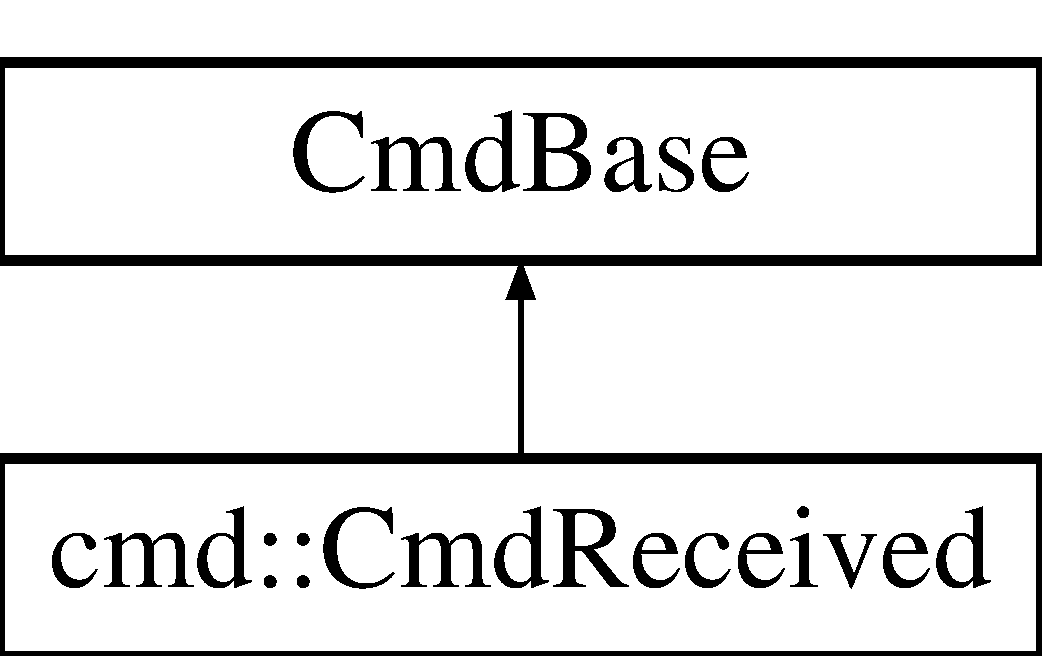
\includegraphics[height=2.000000cm]{classcmd_1_1_cmd_received}
\end{center}
\end{figure}
\subsection*{Public Member Functions}
\begin{DoxyCompactItemize}
\item 
\hyperlink{classcmd_1_1_cmd_received_a4e2d67c5a9de708c11c35a5ea2b5868a}{Cmd\+Received} (std\+::string command=\char`\"{}\char`\"{}, const char field\+\_\+separator= ',', const char cmd\+\_\+separator= ';', const char esc\+\_\+character= '/')
\item 
virtual \hyperlink{classcmd_1_1_cmd_received_aae3a60edebca81eccf26c132abd334bd}{$\sim$\+Cmd\+Received} ()
\item 
bool \hyperlink{classcmd_1_1_cmd_received_a09f6f7766f89968785c3525e3ce8a625}{parse\+Bool} ()
\item 
void \hyperlink{classcmd_1_1_cmd_received_a5f2ae1ffa5dd5312ec12c6e9a46ff24b}{parse\+Bool} (bool \&arg)
\item 
int \hyperlink{classcmd_1_1_cmd_received_a267e265e7bdf5f5e45c1153d78ca0223}{parse\+Int} ()
\item 
void \hyperlink{classcmd_1_1_cmd_received_a8bb8b048253bee5f092d9edd67f8b981}{parse\+Int} (int \&arg)
\item 
char \hyperlink{classcmd_1_1_cmd_received_a7f97a4443af5819d8bcd69e5c51cc4f0}{parse\+Char} ()
\item 
void \hyperlink{classcmd_1_1_cmd_received_a842709f94d709973b62bbd74320825a5}{parse\+Char} (char \&arg)
\item 
float \hyperlink{classcmd_1_1_cmd_received_ac29ede9c4b16e3a768b942a602c72f30}{parse\+Float} ()
\item 
void \hyperlink{classcmd_1_1_cmd_received_a6194b57482cf2f9e235821f03c364496}{parse\+Float} (float \&arg)
\item 
double \hyperlink{classcmd_1_1_cmd_received_a181d947566bb4a9e21725a4e99588c1f}{parse\+Double} ()
\item 
void \hyperlink{classcmd_1_1_cmd_received_a8866107ea61e761416948066b428e54f}{parse\+Double} (double \&arg)
\item 
std\+::string \hyperlink{classcmd_1_1_cmd_received_adf3bc587f2a9b3007b4a5e447116a871}{parse\+String} ()
\item 
void \hyperlink{classcmd_1_1_cmd_received_ad0a14bef5f41acdbe3dba8369fdc015a}{parse\+String} (std\+::string \&arg)
\item 
bool \hyperlink{classcmd_1_1_cmd_received_aff6110aee1a7f6f4f4c0d1542e6cec44}{is\+Valid} ()
\item 
int \hyperlink{classcmd_1_1_cmd_received_af5b660106fb59805494bbb733d1ca5ff}{get\+Num\+Args} ()
\end{DoxyCompactItemize}


\subsection{Detailed Description}


Definition at line 46 of file Cmd\+Received.\+h.



\subsection{Constructor \& Destructor Documentation}
\hypertarget{classcmd_1_1_cmd_received_a4e2d67c5a9de708c11c35a5ea2b5868a}{\index{cmd\+::\+Cmd\+Received@{cmd\+::\+Cmd\+Received}!Cmd\+Received@{Cmd\+Received}}
\index{Cmd\+Received@{Cmd\+Received}!cmd\+::\+Cmd\+Received@{cmd\+::\+Cmd\+Received}}
\subsubsection[{Cmd\+Received}]{\setlength{\rightskip}{0pt plus 5cm}Cmd\+Received\+::\+Cmd\+Received (
\begin{DoxyParamCaption}
\item[{std\+::string}]{command = {\ttfamily \char`\"{}\char`\"{}}, }
\item[{const char}]{field\+\_\+separator = {\ttfamily ','}, }
\item[{const char}]{cmd\+\_\+separator = {\ttfamily ';'}, }
\item[{const char}]{esc\+\_\+character = {\ttfamily '/'}}
\end{DoxyParamCaption}
)}}\label{classcmd_1_1_cmd_received_a4e2d67c5a9de708c11c35a5ea2b5868a}


Definition at line 15 of file Cmd\+Received.\+cpp.

\hypertarget{classcmd_1_1_cmd_received_aae3a60edebca81eccf26c132abd334bd}{\index{cmd\+::\+Cmd\+Received@{cmd\+::\+Cmd\+Received}!````~Cmd\+Received@{$\sim$\+Cmd\+Received}}
\index{````~Cmd\+Received@{$\sim$\+Cmd\+Received}!cmd\+::\+Cmd\+Received@{cmd\+::\+Cmd\+Received}}
\subsubsection[{$\sim$\+Cmd\+Received}]{\setlength{\rightskip}{0pt plus 5cm}Cmd\+Received\+::$\sim$\+Cmd\+Received (
\begin{DoxyParamCaption}
{}
\end{DoxyParamCaption}
)\hspace{0.3cm}{\ttfamily [virtual]}}}\label{classcmd_1_1_cmd_received_aae3a60edebca81eccf26c132abd334bd}


Definition at line 61 of file Cmd\+Received.\+cpp.



\subsection{Member Function Documentation}
\hypertarget{classcmd_1_1_cmd_received_af5b660106fb59805494bbb733d1ca5ff}{\index{cmd\+::\+Cmd\+Received@{cmd\+::\+Cmd\+Received}!get\+Num\+Args@{get\+Num\+Args}}
\index{get\+Num\+Args@{get\+Num\+Args}!cmd\+::\+Cmd\+Received@{cmd\+::\+Cmd\+Received}}
\subsubsection[{get\+Num\+Args}]{\setlength{\rightskip}{0pt plus 5cm}int Cmd\+Received\+::get\+Num\+Args (
\begin{DoxyParamCaption}
{}
\end{DoxyParamCaption}
)}}\label{classcmd_1_1_cmd_received_af5b660106fb59805494bbb733d1ca5ff}
Get the number of arguments left in the queue.

\begin{DoxyReturn}{Returns}
An int representing the number of arguments left. 
\end{DoxyReturn}


Definition at line 250 of file Cmd\+Received.\+cpp.

\hypertarget{classcmd_1_1_cmd_received_aff6110aee1a7f6f4f4c0d1542e6cec44}{\index{cmd\+::\+Cmd\+Received@{cmd\+::\+Cmd\+Received}!is\+Valid@{is\+Valid}}
\index{is\+Valid@{is\+Valid}!cmd\+::\+Cmd\+Received@{cmd\+::\+Cmd\+Received}}
\subsubsection[{is\+Valid}]{\setlength{\rightskip}{0pt plus 5cm}bool Cmd\+Received\+::is\+Valid (
\begin{DoxyParamCaption}
{}
\end{DoxyParamCaption}
)}}\label{classcmd_1_1_cmd_received_aff6110aee1a7f6f4f4c0d1542e6cec44}
Verifies the validity of the received command.

\begin{DoxyReturn}{Returns}
A boolean. True if the command is valid and false otherwise. 
\end{DoxyReturn}


Definition at line 245 of file Cmd\+Received.\+cpp.

\hypertarget{classcmd_1_1_cmd_received_a09f6f7766f89968785c3525e3ce8a625}{\index{cmd\+::\+Cmd\+Received@{cmd\+::\+Cmd\+Received}!parse\+Bool@{parse\+Bool}}
\index{parse\+Bool@{parse\+Bool}!cmd\+::\+Cmd\+Received@{cmd\+::\+Cmd\+Received}}
\subsubsection[{parse\+Bool}]{\setlength{\rightskip}{0pt plus 5cm}bool Cmd\+Received\+::parse\+Bool (
\begin{DoxyParamCaption}
{}
\end{DoxyParamCaption}
)}}\label{classcmd_1_1_cmd_received_a09f6f7766f89968785c3525e3ce8a625}


Definition at line 67 of file Cmd\+Received.\+cpp.

\hypertarget{classcmd_1_1_cmd_received_a5f2ae1ffa5dd5312ec12c6e9a46ff24b}{\index{cmd\+::\+Cmd\+Received@{cmd\+::\+Cmd\+Received}!parse\+Bool@{parse\+Bool}}
\index{parse\+Bool@{parse\+Bool}!cmd\+::\+Cmd\+Received@{cmd\+::\+Cmd\+Received}}
\subsubsection[{parse\+Bool}]{\setlength{\rightskip}{0pt plus 5cm}void Cmd\+Received\+::parse\+Bool (
\begin{DoxyParamCaption}
\item[{bool \&}]{arg}
\end{DoxyParamCaption}
)}}\label{classcmd_1_1_cmd_received_a5f2ae1ffa5dd5312ec12c6e9a46ff24b}
Parses the next argument as a bool.


\begin{DoxyParams}{Parameters}
{\em arg} & Reference of a bool to receive the parsed argument. \\
\hline
\end{DoxyParams}


Definition at line 87 of file Cmd\+Received.\+cpp.

\hypertarget{classcmd_1_1_cmd_received_a7f97a4443af5819d8bcd69e5c51cc4f0}{\index{cmd\+::\+Cmd\+Received@{cmd\+::\+Cmd\+Received}!parse\+Char@{parse\+Char}}
\index{parse\+Char@{parse\+Char}!cmd\+::\+Cmd\+Received@{cmd\+::\+Cmd\+Received}}
\subsubsection[{parse\+Char}]{\setlength{\rightskip}{0pt plus 5cm}char Cmd\+Received\+::parse\+Char (
\begin{DoxyParamCaption}
{}
\end{DoxyParamCaption}
)}}\label{classcmd_1_1_cmd_received_a7f97a4443af5819d8bcd69e5c51cc4f0}
Parses the next argument as a character.

\begin{DoxyReturn}{Returns}
A character representing the parsed argument. 
\end{DoxyReturn}


Definition at line 136 of file Cmd\+Received.\+cpp.

\hypertarget{classcmd_1_1_cmd_received_a842709f94d709973b62bbd74320825a5}{\index{cmd\+::\+Cmd\+Received@{cmd\+::\+Cmd\+Received}!parse\+Char@{parse\+Char}}
\index{parse\+Char@{parse\+Char}!cmd\+::\+Cmd\+Received@{cmd\+::\+Cmd\+Received}}
\subsubsection[{parse\+Char}]{\setlength{\rightskip}{0pt plus 5cm}void Cmd\+Received\+::parse\+Char (
\begin{DoxyParamCaption}
\item[{char \&}]{arg}
\end{DoxyParamCaption}
)}}\label{classcmd_1_1_cmd_received_a842709f94d709973b62bbd74320825a5}
Parses the next argument as a character.


\begin{DoxyParams}{Parameters}
{\em arg} & Reference of a character to receive the parsed argument. \\
\hline
\end{DoxyParams}


Definition at line 156 of file Cmd\+Received.\+cpp.

\hypertarget{classcmd_1_1_cmd_received_a181d947566bb4a9e21725a4e99588c1f}{\index{cmd\+::\+Cmd\+Received@{cmd\+::\+Cmd\+Received}!parse\+Double@{parse\+Double}}
\index{parse\+Double@{parse\+Double}!cmd\+::\+Cmd\+Received@{cmd\+::\+Cmd\+Received}}
\subsubsection[{parse\+Double}]{\setlength{\rightskip}{0pt plus 5cm}double Cmd\+Received\+::parse\+Double (
\begin{DoxyParamCaption}
{}
\end{DoxyParamCaption}
)}}\label{classcmd_1_1_cmd_received_a181d947566bb4a9e21725a4e99588c1f}
Parses the next argument as a double.

\begin{DoxyReturn}{Returns}
A double representing the parsed argument. 
\end{DoxyReturn}


Definition at line 200 of file Cmd\+Received.\+cpp.

\hypertarget{classcmd_1_1_cmd_received_a8866107ea61e761416948066b428e54f}{\index{cmd\+::\+Cmd\+Received@{cmd\+::\+Cmd\+Received}!parse\+Double@{parse\+Double}}
\index{parse\+Double@{parse\+Double}!cmd\+::\+Cmd\+Received@{cmd\+::\+Cmd\+Received}}
\subsubsection[{parse\+Double}]{\setlength{\rightskip}{0pt plus 5cm}void Cmd\+Received\+::parse\+Double (
\begin{DoxyParamCaption}
\item[{double \&}]{arg}
\end{DoxyParamCaption}
)}}\label{classcmd_1_1_cmd_received_a8866107ea61e761416948066b428e54f}
Parses the next argument as a double.


\begin{DoxyParams}{Parameters}
{\em arg} & Reference of a double to receive the parsed argument. \\
\hline
\end{DoxyParams}


Definition at line 217 of file Cmd\+Received.\+cpp.

\hypertarget{classcmd_1_1_cmd_received_ac29ede9c4b16e3a768b942a602c72f30}{\index{cmd\+::\+Cmd\+Received@{cmd\+::\+Cmd\+Received}!parse\+Float@{parse\+Float}}
\index{parse\+Float@{parse\+Float}!cmd\+::\+Cmd\+Received@{cmd\+::\+Cmd\+Received}}
\subsubsection[{parse\+Float}]{\setlength{\rightskip}{0pt plus 5cm}float Cmd\+Received\+::parse\+Float (
\begin{DoxyParamCaption}
{}
\end{DoxyParamCaption}
)}}\label{classcmd_1_1_cmd_received_ac29ede9c4b16e3a768b942a602c72f30}
Parses the next argument as a float.

\begin{DoxyReturn}{Returns}
A float representing the parsed argument. 
\end{DoxyReturn}


Definition at line 171 of file Cmd\+Received.\+cpp.

\hypertarget{classcmd_1_1_cmd_received_a6194b57482cf2f9e235821f03c364496}{\index{cmd\+::\+Cmd\+Received@{cmd\+::\+Cmd\+Received}!parse\+Float@{parse\+Float}}
\index{parse\+Float@{parse\+Float}!cmd\+::\+Cmd\+Received@{cmd\+::\+Cmd\+Received}}
\subsubsection[{parse\+Float}]{\setlength{\rightskip}{0pt plus 5cm}void Cmd\+Received\+::parse\+Float (
\begin{DoxyParamCaption}
\item[{float \&}]{arg}
\end{DoxyParamCaption}
)}}\label{classcmd_1_1_cmd_received_a6194b57482cf2f9e235821f03c364496}
Parses the next argument as a float.

arg Reference of a float to receive the parsed argument. 

Definition at line 188 of file Cmd\+Received.\+cpp.

\hypertarget{classcmd_1_1_cmd_received_a267e265e7bdf5f5e45c1153d78ca0223}{\index{cmd\+::\+Cmd\+Received@{cmd\+::\+Cmd\+Received}!parse\+Int@{parse\+Int}}
\index{parse\+Int@{parse\+Int}!cmd\+::\+Cmd\+Received@{cmd\+::\+Cmd\+Received}}
\subsubsection[{parse\+Int}]{\setlength{\rightskip}{0pt plus 5cm}int Cmd\+Received\+::parse\+Int (
\begin{DoxyParamCaption}
{}
\end{DoxyParamCaption}
)}}\label{classcmd_1_1_cmd_received_a267e265e7bdf5f5e45c1153d78ca0223}
Parses the next argument as an integer.

\begin{DoxyReturn}{Returns}
An integer representing the parsed argument. 
\end{DoxyReturn}


Definition at line 101 of file Cmd\+Received.\+cpp.

\hypertarget{classcmd_1_1_cmd_received_a8bb8b048253bee5f092d9edd67f8b981}{\index{cmd\+::\+Cmd\+Received@{cmd\+::\+Cmd\+Received}!parse\+Int@{parse\+Int}}
\index{parse\+Int@{parse\+Int}!cmd\+::\+Cmd\+Received@{cmd\+::\+Cmd\+Received}}
\subsubsection[{parse\+Int}]{\setlength{\rightskip}{0pt plus 5cm}void Cmd\+Received\+::parse\+Int (
\begin{DoxyParamCaption}
\item[{int \&}]{arg}
\end{DoxyParamCaption}
)}}\label{classcmd_1_1_cmd_received_a8bb8b048253bee5f092d9edd67f8b981}
Parses the next argument as an integer.


\begin{DoxyParams}{Parameters}
{\em arg} & Reference of an integer to receive the parsed argument. \\
\hline
\end{DoxyParams}


Definition at line 121 of file Cmd\+Received.\+cpp.

\hypertarget{classcmd_1_1_cmd_received_adf3bc587f2a9b3007b4a5e447116a871}{\index{cmd\+::\+Cmd\+Received@{cmd\+::\+Cmd\+Received}!parse\+String@{parse\+String}}
\index{parse\+String@{parse\+String}!cmd\+::\+Cmd\+Received@{cmd\+::\+Cmd\+Received}}
\subsubsection[{parse\+String}]{\setlength{\rightskip}{0pt plus 5cm}std\+::string Cmd\+Received\+::parse\+String (
\begin{DoxyParamCaption}
{}
\end{DoxyParamCaption}
)}}\label{classcmd_1_1_cmd_received_adf3bc587f2a9b3007b4a5e447116a871}
Parses the next argument as a String.

\begin{DoxyReturn}{Returns}
A std\+::string representing the parsed argument. 
\end{DoxyReturn}


Definition at line 229 of file Cmd\+Received.\+cpp.

\hypertarget{classcmd_1_1_cmd_received_ad0a14bef5f41acdbe3dba8369fdc015a}{\index{cmd\+::\+Cmd\+Received@{cmd\+::\+Cmd\+Received}!parse\+String@{parse\+String}}
\index{parse\+String@{parse\+String}!cmd\+::\+Cmd\+Received@{cmd\+::\+Cmd\+Received}}
\subsubsection[{parse\+String}]{\setlength{\rightskip}{0pt plus 5cm}void Cmd\+Received\+::parse\+String (
\begin{DoxyParamCaption}
\item[{std\+::string \&}]{arg}
\end{DoxyParamCaption}
)}}\label{classcmd_1_1_cmd_received_ad0a14bef5f41acdbe3dba8369fdc015a}
Parses the next argument as a String.


\begin{DoxyParams}{Parameters}
{\em arg} & Reference of a std\+::string to receive the parsed argument. \\
\hline
\end{DoxyParams}


Definition at line 237 of file Cmd\+Received.\+cpp.



The documentation for this class was generated from the following files\+:\begin{DoxyCompactItemize}
\item 
/home/edno/projetos/cmd\+Messenger-\/cpp/include/\hyperlink{_cmd_received_8h}{Cmd\+Received.\+h}\item 
/home/edno/projetos/cmd\+Messenger-\/cpp/src/\hyperlink{_cmd_received_8cpp}{Cmd\+Received.\+cpp}\end{DoxyCompactItemize}

\hypertarget{classcmd_1_1_cmd_send}{\section{cmd\+:\+:Cmd\+Send Class Reference}
\label{classcmd_1_1_cmd_send}\index{cmd\+::\+Cmd\+Send@{cmd\+::\+Cmd\+Send}}
}


{\ttfamily \#include $<$Cmd\+Send.\+h$>$}

Inheritance diagram for cmd\+:\+:Cmd\+Send\+:\begin{figure}[H]
\begin{center}
\leavevmode
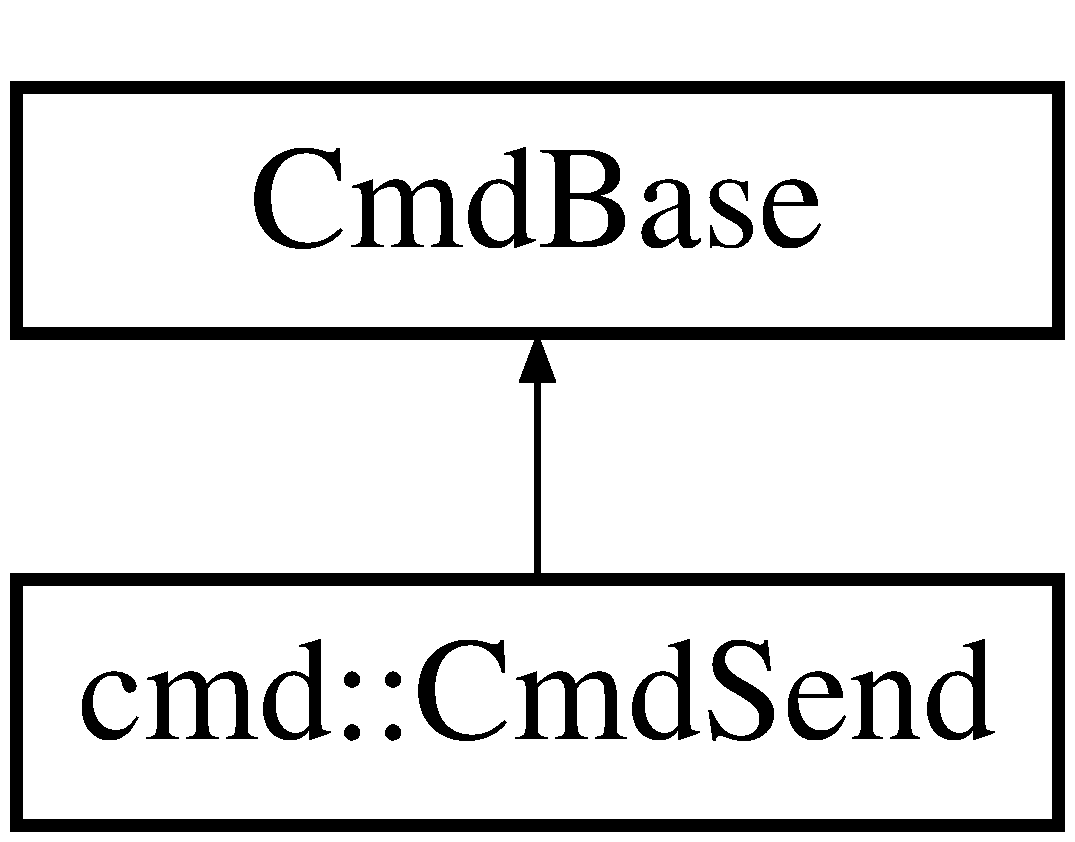
\includegraphics[height=2.000000cm]{classcmd_1_1_cmd_send}
\end{center}
\end{figure}
\subsection*{Public Member Functions}
\begin{DoxyCompactItemize}
\item 
\hyperlink{classcmd_1_1_cmd_send_a0bde526ff8e0d36be47f2ad4f614be99}{Cmd\+Send} (int id=0)
\item 
virtual \hyperlink{classcmd_1_1_cmd_send_abf939f6219c5c5d5e5caf59d36b7d3ed}{$\sim$\+Cmd\+Send} ()
\item 
{\footnotesize template$<$typename T $>$ }\\void \hyperlink{classcmd_1_1_cmd_send_adf3459b9e64391790a844ade051a07eb}{add} (T arg)
\item 
void \hyperlink{classcmd_1_1_cmd_send_a189a3db925e6be886c787c1206846b1a}{add} (\hyperlink{class_cmd_end}{Cmd\+End} end)
\item 
{\footnotesize template$<$typename T $>$ }\\\hyperlink{classcmd_1_1_cmd_send}{Cmd\+Send} \& \hyperlink{classcmd_1_1_cmd_send_a4c90185bdf7ed1b3442bd69a2a9cd5b2}{operator$<$$<$} (T arg)
\item 
void \hyperlink{classcmd_1_1_cmd_send_ae11b3feb18c2b48113ad048c7f2bda2e}{operator$<$$<$} (\hyperlink{class_cmd_end}{Cmd\+End} end)
\item 
void \hyperlink{classcmd_1_1_cmd_send_abefba8ff2e9c9c2e13c3ccda96a34e32}{clear} ()
\item 
bool \hyperlink{classcmd_1_1_cmd_send_a2906af83411722ad6ca6d074e3155396}{get\+State} () const 
\item 
int \hyperlink{classcmd_1_1_cmd_send_a0434b09f3aa8ad368b043163edff3e44}{get\+Num\+Args} () const 
\end{DoxyCompactItemize}
\subsection*{Friends}
\begin{DoxyCompactItemize}
\item 
class \hyperlink{classcmd_1_1_cmd_send_aec8a96be1b821d4fc3138f1840a757c9}{Cmd\+Messenger}
\end{DoxyCompactItemize}


\subsection{Detailed Description}


Definition at line 48 of file Cmd\+Send.\+h.



\subsection{Constructor \& Destructor Documentation}
\hypertarget{classcmd_1_1_cmd_send_a0bde526ff8e0d36be47f2ad4f614be99}{\index{cmd\+::\+Cmd\+Send@{cmd\+::\+Cmd\+Send}!Cmd\+Send@{Cmd\+Send}}
\index{Cmd\+Send@{Cmd\+Send}!cmd\+::\+Cmd\+Send@{cmd\+::\+Cmd\+Send}}
\subsubsection[{Cmd\+Send}]{\setlength{\rightskip}{0pt plus 5cm}Cmd\+Send\+::\+Cmd\+Send (
\begin{DoxyParamCaption}
\item[{int}]{id = {\ttfamily 0}}
\end{DoxyParamCaption}
)}}\label{classcmd_1_1_cmd_send_a0bde526ff8e0d36be47f2ad4f614be99}


Definition at line 8 of file Cmd\+Send.\+cpp.

\hypertarget{classcmd_1_1_cmd_send_abf939f6219c5c5d5e5caf59d36b7d3ed}{\index{cmd\+::\+Cmd\+Send@{cmd\+::\+Cmd\+Send}!````~Cmd\+Send@{$\sim$\+Cmd\+Send}}
\index{````~Cmd\+Send@{$\sim$\+Cmd\+Send}!cmd\+::\+Cmd\+Send@{cmd\+::\+Cmd\+Send}}
\subsubsection[{$\sim$\+Cmd\+Send}]{\setlength{\rightskip}{0pt plus 5cm}Cmd\+Send\+::$\sim$\+Cmd\+Send (
\begin{DoxyParamCaption}
{}
\end{DoxyParamCaption}
)\hspace{0.3cm}{\ttfamily [virtual]}}}\label{classcmd_1_1_cmd_send_abf939f6219c5c5d5e5caf59d36b7d3ed}


Definition at line 14 of file Cmd\+Send.\+cpp.



\subsection{Member Function Documentation}
\hypertarget{classcmd_1_1_cmd_send_adf3459b9e64391790a844ade051a07eb}{\index{cmd\+::\+Cmd\+Send@{cmd\+::\+Cmd\+Send}!add@{add}}
\index{add@{add}!cmd\+::\+Cmd\+Send@{cmd\+::\+Cmd\+Send}}
\subsubsection[{add}]{\setlength{\rightskip}{0pt plus 5cm}template$<$typename T $>$ void cmd\+::\+Cmd\+Send\+::add (
\begin{DoxyParamCaption}
\item[{T}]{arg}
\end{DoxyParamCaption}
)\hspace{0.3cm}{\ttfamily [inline]}}}\label{classcmd_1_1_cmd_send_adf3459b9e64391790a844ade051a07eb}


Definition at line 58 of file Cmd\+Send.\+h.

\hypertarget{classcmd_1_1_cmd_send_a189a3db925e6be886c787c1206846b1a}{\index{cmd\+::\+Cmd\+Send@{cmd\+::\+Cmd\+Send}!add@{add}}
\index{add@{add}!cmd\+::\+Cmd\+Send@{cmd\+::\+Cmd\+Send}}
\subsubsection[{add}]{\setlength{\rightskip}{0pt plus 5cm}void Cmd\+Send\+::add (
\begin{DoxyParamCaption}
\item[{{\bf Cmd\+End}}]{end}
\end{DoxyParamCaption}
)}}\label{classcmd_1_1_cmd_send_a189a3db925e6be886c787c1206846b1a}


Definition at line 18 of file Cmd\+Send.\+cpp.

\hypertarget{classcmd_1_1_cmd_send_abefba8ff2e9c9c2e13c3ccda96a34e32}{\index{cmd\+::\+Cmd\+Send@{cmd\+::\+Cmd\+Send}!clear@{clear}}
\index{clear@{clear}!cmd\+::\+Cmd\+Send@{cmd\+::\+Cmd\+Send}}
\subsubsection[{clear}]{\setlength{\rightskip}{0pt plus 5cm}void Cmd\+Send\+::clear (
\begin{DoxyParamCaption}
{}
\end{DoxyParamCaption}
)}}\label{classcmd_1_1_cmd_send_abefba8ff2e9c9c2e13c3ccda96a34e32}


Definition at line 38 of file Cmd\+Send.\+cpp.

\hypertarget{classcmd_1_1_cmd_send_a0434b09f3aa8ad368b043163edff3e44}{\index{cmd\+::\+Cmd\+Send@{cmd\+::\+Cmd\+Send}!get\+Num\+Args@{get\+Num\+Args}}
\index{get\+Num\+Args@{get\+Num\+Args}!cmd\+::\+Cmd\+Send@{cmd\+::\+Cmd\+Send}}
\subsubsection[{get\+Num\+Args}]{\setlength{\rightskip}{0pt plus 5cm}int Cmd\+Send\+::get\+Num\+Args (
\begin{DoxyParamCaption}
{}
\end{DoxyParamCaption}
) const}}\label{classcmd_1_1_cmd_send_a0434b09f3aa8ad368b043163edff3e44}


Definition at line 33 of file Cmd\+Send.\+cpp.

\hypertarget{classcmd_1_1_cmd_send_a2906af83411722ad6ca6d074e3155396}{\index{cmd\+::\+Cmd\+Send@{cmd\+::\+Cmd\+Send}!get\+State@{get\+State}}
\index{get\+State@{get\+State}!cmd\+::\+Cmd\+Send@{cmd\+::\+Cmd\+Send}}
\subsubsection[{get\+State}]{\setlength{\rightskip}{0pt plus 5cm}bool Cmd\+Send\+::get\+State (
\begin{DoxyParamCaption}
{}
\end{DoxyParamCaption}
) const}}\label{classcmd_1_1_cmd_send_a2906af83411722ad6ca6d074e3155396}
Gets the state of the command.

\begin{DoxyReturn}{Returns}
A bool that represents the state. True if the command is ready to be sent and false if it is not. 
\end{DoxyReturn}


Definition at line 28 of file Cmd\+Send.\+cpp.

\hypertarget{classcmd_1_1_cmd_send_a4c90185bdf7ed1b3442bd69a2a9cd5b2}{\index{cmd\+::\+Cmd\+Send@{cmd\+::\+Cmd\+Send}!operator$<$$<$@{operator$<$$<$}}
\index{operator$<$$<$@{operator$<$$<$}!cmd\+::\+Cmd\+Send@{cmd\+::\+Cmd\+Send}}
\subsubsection[{operator$<$$<$}]{\setlength{\rightskip}{0pt plus 5cm}template$<$typename T $>$ {\bf Cmd\+Send}\& cmd\+::\+Cmd\+Send\+::operator$<$$<$ (
\begin{DoxyParamCaption}
\item[{T}]{arg}
\end{DoxyParamCaption}
)\hspace{0.3cm}{\ttfamily [inline]}}}\label{classcmd_1_1_cmd_send_a4c90185bdf7ed1b3442bd69a2a9cd5b2}


Definition at line 70 of file Cmd\+Send.\+h.

\hypertarget{classcmd_1_1_cmd_send_ae11b3feb18c2b48113ad048c7f2bda2e}{\index{cmd\+::\+Cmd\+Send@{cmd\+::\+Cmd\+Send}!operator$<$$<$@{operator$<$$<$}}
\index{operator$<$$<$@{operator$<$$<$}!cmd\+::\+Cmd\+Send@{cmd\+::\+Cmd\+Send}}
\subsubsection[{operator$<$$<$}]{\setlength{\rightskip}{0pt plus 5cm}void Cmd\+Send\+::operator$<$$<$ (
\begin{DoxyParamCaption}
\item[{{\bf Cmd\+End}}]{end}
\end{DoxyParamCaption}
)}}\label{classcmd_1_1_cmd_send_ae11b3feb18c2b48113ad048c7f2bda2e}


Definition at line 23 of file Cmd\+Send.\+cpp.



\subsection{Friends And Related Function Documentation}
\hypertarget{classcmd_1_1_cmd_send_aec8a96be1b821d4fc3138f1840a757c9}{\index{cmd\+::\+Cmd\+Send@{cmd\+::\+Cmd\+Send}!Cmd\+Messenger@{Cmd\+Messenger}}
\index{Cmd\+Messenger@{Cmd\+Messenger}!cmd\+::\+Cmd\+Send@{cmd\+::\+Cmd\+Send}}
\subsubsection[{Cmd\+Messenger}]{\setlength{\rightskip}{0pt plus 5cm}friend class {\bf Cmd\+Messenger}\hspace{0.3cm}{\ttfamily [friend]}}}\label{classcmd_1_1_cmd_send_aec8a96be1b821d4fc3138f1840a757c9}


Definition at line 100 of file Cmd\+Send.\+h.



The documentation for this class was generated from the following files\+:\begin{DoxyCompactItemize}
\item 
/home/edno/projetos/robot/cmd\+Messenger-\/cpp/include/\hyperlink{_cmd_send_8h}{Cmd\+Send.\+h}\item 
/home/edno/projetos/robot/cmd\+Messenger-\/cpp/src/\hyperlink{_cmd_send_8cpp}{Cmd\+Send.\+cpp}\end{DoxyCompactItemize}

\chapter{File Documentation}
\hypertarget{main_8dox}{\section{main.\+dox File Reference}
\label{main_8dox}\index{main.\+dox@{main.\+dox}}
}

\hypertarget{_cmd_base_8h}{\section{/home/edno/projetos/robot/cmd\+Messenger-\/cpp/include/\+Cmd\+Base.h File Reference}
\label{_cmd_base_8h}\index{/home/edno/projetos/robot/cmd\+Messenger-\/cpp/include/\+Cmd\+Base.\+h@{/home/edno/projetos/robot/cmd\+Messenger-\/cpp/include/\+Cmd\+Base.\+h}}
}
\subsection*{Data Structures}
\begin{DoxyCompactItemize}
\item 
class \hyperlink{class_cmd_end}{Cmd\+End}
\item 
class \hyperlink{class_cmd_base}{Cmd\+Base}
\end{DoxyCompactItemize}


\subsection{Detailed Description}
\begin{DoxyAuthor}{Author}
Rodrigues Filho 
\end{DoxyAuthor}
\begin{DoxyVersion}{Version}
0.\+1
\end{DoxyVersion}
\hypertarget{_cmd_messenger_8cpp_LICENSE}{}\subsection{L\+I\+C\+E\+N\+S\+E}\label{_cmd_messenger_8cpp_LICENSE}
The M\+I\+T License

Copyright (c) 2014 Francisco Edno de Moura Rodrigues Filho

Permission is hereby granted, free of charge, to any person obtaining a copy of this software and associated documentation files (the \char`\"{}\+Software\char`\"{}), to deal in the Software without restriction, including without limitation the rights to use, copy, modify, merge, publish, distribute, sublicense, and/or sell copies of the Software, and to permit persons to whom the Software is furnished to do so, subject to the following conditions\+:

The above copyright notice and this permission notice shall be included in all copies or substantial portions of the Software.

T\+H\+E S\+O\+F\+T\+W\+A\+R\+E I\+S P\+R\+O\+V\+I\+D\+E\+D \char`\"{}\+A\+S I\+S\char`\"{}, W\+I\+T\+H\+O\+U\+T W\+A\+R\+R\+A\+N\+T\+Y O\+F A\+N\+Y K\+I\+N\+D, E\+X\+P\+R\+E\+S\+S O\+R I\+M\+P\+L\+I\+E\+D, I\+N\+C\+L\+U\+D\+I\+N\+G B\+U\+T N\+O\+T L\+I\+M\+I\+T\+E\+D T\+O T\+H\+E W\+A\+R\+R\+A\+N\+T\+I\+E\+S O\+F M\+E\+R\+C\+H\+A\+N\+T\+A\+B\+I\+L\+I\+T\+Y, F\+I\+T\+N\+E\+S\+S F\+O\+R A P\+A\+R\+T\+I\+C\+U\+L\+A\+R P\+U\+R\+P\+O\+S\+E A\+N\+D N\+O\+N\+I\+N\+F\+R\+I\+N\+G\+E\+M\+E\+N\+T. I\+N N\+O E\+V\+E\+N\+T S\+H\+A\+L\+L T\+H\+E A\+U\+T\+H\+O\+R\+S O\+R C\+O\+P\+Y\+R\+I\+G\+H\+T H\+O\+L\+D\+E\+R\+S B\+E L\+I\+A\+B\+L\+E F\+O\+R A\+N\+Y C\+L\+A\+I\+M, D\+A\+M\+A\+G\+E\+S O\+R O\+T\+H\+E\+R L\+I\+A\+B\+I\+L\+I\+T\+Y, W\+H\+E\+T\+H\+E\+R I\+N A\+N A\+C\+T\+I\+O\+N O\+F C\+O\+N\+T\+R\+A\+C\+T, T\+O\+R\+T O\+R O\+T\+H\+E\+R\+W\+I\+S\+E, A\+R\+I\+S\+I\+N\+G F\+R\+O\+M, O\+U\+T O\+F O\+R I\+N C\+O\+N\+N\+E\+C\+T\+I\+O\+N W\+I\+T\+H T\+H\+E S\+O\+F\+T\+W\+A\+R\+E O\+R T\+H\+E U\+S\+E O\+R O\+T\+H\+E\+R D\+E\+A\+L\+I\+N\+G\+S I\+N T\+H\+E S\+O\+F\+T\+W\+A\+R\+E.\hypertarget{_cmd_received_8h_DESCRIPTION}{}\subsection{D\+E\+S\+C\+R\+I\+P\+T\+I\+O\+N}\label{_cmd_received_8h_DESCRIPTION}
This provides a base interface for commands in this Cmd\+Messenger C++ implementation. Here, the empty class \hyperlink{class_cmd_end}{Cmd\+End} is also defined. 

Definition in file \hyperlink{_cmd_base_8h_source}{Cmd\+Base.\+h}.


\hypertarget{_cmd_messenger_8h}{\section{/home/edno/projetos/robot/cmd\+Messenger-\/cpp/include/\+Cmd\+Messenger.h File Reference}
\label{_cmd_messenger_8h}\index{/home/edno/projetos/robot/cmd\+Messenger-\/cpp/include/\+Cmd\+Messenger.\+h@{/home/edno/projetos/robot/cmd\+Messenger-\/cpp/include/\+Cmd\+Messenger.\+h}}
}
{\ttfamily \#include $<$iostream$>$}\\*
{\ttfamily \#include $<$map$>$}\\*
{\ttfamily \#include \char`\"{}serial/serial.\+h\char`\"{}}\\*
{\ttfamily \#include \char`\"{}callback.\+h\char`\"{}}\\*
{\ttfamily \#include \char`\"{}Cmd\+Send.\+h\char`\"{}}\\*
{\ttfamily \#include \char`\"{}Cmd\+Received.\+h\char`\"{}}\\*
\subsection*{Data Structures}
\begin{DoxyCompactItemize}
\item 
class \hyperlink{classcmd_1_1_cmd_messenger}{cmd\+::\+Cmd\+Messenger}
\end{DoxyCompactItemize}
\subsection*{Namespaces}
\begin{DoxyCompactItemize}
\item 
 \hyperlink{namespacecmd}{cmd}
\end{DoxyCompactItemize}
\subsection*{Typedefs}
\begin{DoxyCompactItemize}
\item 
typedef Cmd\+Send \hyperlink{namespacecmd_af9b58ca395c80edd1335e21d1b9f4c99}{cmd\+::\+Cmd}
\item 
typedef \hyperlink{class_c_b_functor1w_ret}{C\+B\+Functor1w\+Ret}\\*
$<$ Cmd\+Received \&, void $>$ \hyperlink{namespacecmd_a24926dd0c7587e1961fd9ebe0259beea}{cmd\+::\+Call\+Back\+Functor}
\item 
typedef void($\ast$ \hyperlink{namespacecmd_a20b40ecd3ba46130eef6c125f70c4121}{cmd\+::\+Call\+Back} )(Cmd\+Received \&)
\end{DoxyCompactItemize}


\subsection{Detailed Description}
\begin{DoxyAuthor}{Author}
Rodrigues Filho 
\end{DoxyAuthor}
\begin{DoxyVersion}{Version}
0.\+1
\end{DoxyVersion}
\hypertarget{_cmd_messenger_8cpp_LICENSE}{}\subsection{L\+I\+C\+E\+N\+S\+E}\label{_cmd_messenger_8cpp_LICENSE}
The M\+I\+T License

Copyright (c) 2014 Francisco Edno de Moura Rodrigues Filho

Permission is hereby granted, free of charge, to any person obtaining a copy of this software and associated documentation files (the \char`\"{}\+Software\char`\"{}), to deal in the Software without restriction, including without limitation the rights to use, copy, modify, merge, publish, distribute, sublicense, and/or sell copies of the Software, and to permit persons to whom the Software is furnished to do so, subject to the following conditions\+:

The above copyright notice and this permission notice shall be included in all copies or substantial portions of the Software.

T\+H\+E S\+O\+F\+T\+W\+A\+R\+E I\+S P\+R\+O\+V\+I\+D\+E\+D \char`\"{}\+A\+S I\+S\char`\"{}, W\+I\+T\+H\+O\+U\+T W\+A\+R\+R\+A\+N\+T\+Y O\+F A\+N\+Y K\+I\+N\+D, E\+X\+P\+R\+E\+S\+S O\+R I\+M\+P\+L\+I\+E\+D, I\+N\+C\+L\+U\+D\+I\+N\+G B\+U\+T N\+O\+T L\+I\+M\+I\+T\+E\+D T\+O T\+H\+E W\+A\+R\+R\+A\+N\+T\+I\+E\+S O\+F M\+E\+R\+C\+H\+A\+N\+T\+A\+B\+I\+L\+I\+T\+Y, F\+I\+T\+N\+E\+S\+S F\+O\+R A P\+A\+R\+T\+I\+C\+U\+L\+A\+R P\+U\+R\+P\+O\+S\+E A\+N\+D N\+O\+N\+I\+N\+F\+R\+I\+N\+G\+E\+M\+E\+N\+T. I\+N N\+O E\+V\+E\+N\+T S\+H\+A\+L\+L T\+H\+E A\+U\+T\+H\+O\+R\+S O\+R C\+O\+P\+Y\+R\+I\+G\+H\+T H\+O\+L\+D\+E\+R\+S B\+E L\+I\+A\+B\+L\+E F\+O\+R A\+N\+Y C\+L\+A\+I\+M, D\+A\+M\+A\+G\+E\+S O\+R O\+T\+H\+E\+R L\+I\+A\+B\+I\+L\+I\+T\+Y, W\+H\+E\+T\+H\+E\+R I\+N A\+N A\+C\+T\+I\+O\+N O\+F C\+O\+N\+T\+R\+A\+C\+T, T\+O\+R\+T O\+R O\+T\+H\+E\+R\+W\+I\+S\+E, A\+R\+I\+S\+I\+N\+G F\+R\+O\+M, O\+U\+T O\+F O\+R I\+N C\+O\+N\+N\+E\+C\+T\+I\+O\+N W\+I\+T\+H T\+H\+E S\+O\+F\+T\+W\+A\+R\+E O\+R T\+H\+E U\+S\+E O\+R O\+T\+H\+E\+R D\+E\+A\+L\+I\+N\+G\+S I\+N T\+H\+E S\+O\+F\+T\+W\+A\+R\+E.\hypertarget{_cmd_received_8h_DESCRIPTION}{}\subsection{D\+E\+S\+C\+R\+I\+P\+T\+I\+O\+N}\label{_cmd_received_8h_DESCRIPTION}
This provides a cross platform interface to use with the Cmd\+Messenger messaging library. As transport layer the Serial Library, a cross-\/platform, simple to use library for using serial ports on computers by William Woodall (\href{mailto:wjwwood@gmail.com}{\tt wjwwood@gmail.\+com}) and John Harrison (\href{mailto:ash@greaterthaninfinity.com}{\tt ash@greaterthaninfinity.\+com}), was chosen. This is the main interface to use this Cmd\+Messenger implementation. 

Definition in file \hyperlink{_cmd_messenger_8h_source}{Cmd\+Messenger.\+h}.


\hypertarget{_cmd_received_8h}{\section{/home/edno/projetos/cmd\+Messenger-\/cpp/include/\+Cmd\+Received.h File Reference}
\label{_cmd_received_8h}\index{/home/edno/projetos/cmd\+Messenger-\/cpp/include/\+Cmd\+Received.\+h@{/home/edno/projetos/cmd\+Messenger-\/cpp/include/\+Cmd\+Received.\+h}}
}
{\ttfamily \#include $<$iostream$>$}\\*
{\ttfamily \#include $<$queue$>$}\\*
{\ttfamily \#include \char`\"{}Cmd\+Base.\+h\char`\"{}}\\*
\subsection*{Data Structures}
\begin{DoxyCompactItemize}
\item 
class \hyperlink{classcmd_1_1_cmd_received}{cmd\+::\+Cmd\+Received}
\end{DoxyCompactItemize}
\subsection*{Namespaces}
\begin{DoxyCompactItemize}
\item 
 \hyperlink{namespacecmd}{cmd}
\end{DoxyCompactItemize}


\subsection{Detailed Description}
\begin{DoxyAuthor}{Author}
Rodrigues Filho 
\end{DoxyAuthor}
\begin{DoxyVersion}{Version}
0.\+1
\end{DoxyVersion}
\hypertarget{_cmd_messenger_8cpp_LICENSE}{}\subsection{L\+I\+C\+E\+N\+S\+E}\label{_cmd_messenger_8cpp_LICENSE}
The M\+I\+T License

Copyright (c) 2014 Francisco Edno de Moura Rodrigues Filho

Permission is hereby granted, free of charge, to any person obtaining a copy of this software and associated documentation files (the \char`\"{}\+Software\char`\"{}), to deal in the Software without restriction, including without limitation the rights to use, copy, modify, merge, publish, distribute, sublicense, and/or sell copies of the Software, and to permit persons to whom the Software is furnished to do so, subject to the following conditions\+:

The above copyright notice and this permission notice shall be included in all copies or substantial portions of the Software.

T\+H\+E S\+O\+F\+T\+W\+A\+R\+E I\+S P\+R\+O\+V\+I\+D\+E\+D \char`\"{}\+A\+S I\+S\char`\"{}, W\+I\+T\+H\+O\+U\+T W\+A\+R\+R\+A\+N\+T\+Y O\+F A\+N\+Y K\+I\+N\+D, E\+X\+P\+R\+E\+S\+S O\+R I\+M\+P\+L\+I\+E\+D, I\+N\+C\+L\+U\+D\+I\+N\+G B\+U\+T N\+O\+T L\+I\+M\+I\+T\+E\+D T\+O T\+H\+E W\+A\+R\+R\+A\+N\+T\+I\+E\+S O\+F M\+E\+R\+C\+H\+A\+N\+T\+A\+B\+I\+L\+I\+T\+Y, F\+I\+T\+N\+E\+S\+S F\+O\+R A P\+A\+R\+T\+I\+C\+U\+L\+A\+R P\+U\+R\+P\+O\+S\+E A\+N\+D N\+O\+N\+I\+N\+F\+R\+I\+N\+G\+E\+M\+E\+N\+T. I\+N N\+O E\+V\+E\+N\+T S\+H\+A\+L\+L T\+H\+E A\+U\+T\+H\+O\+R\+S O\+R C\+O\+P\+Y\+R\+I\+G\+H\+T H\+O\+L\+D\+E\+R\+S B\+E L\+I\+A\+B\+L\+E F\+O\+R A\+N\+Y C\+L\+A\+I\+M, D\+A\+M\+A\+G\+E\+S O\+R O\+T\+H\+E\+R L\+I\+A\+B\+I\+L\+I\+T\+Y, W\+H\+E\+T\+H\+E\+R I\+N A\+N A\+C\+T\+I\+O\+N O\+F C\+O\+N\+T\+R\+A\+C\+T, T\+O\+R\+T O\+R O\+T\+H\+E\+R\+W\+I\+S\+E, A\+R\+I\+S\+I\+N\+G F\+R\+O\+M, O\+U\+T O\+F O\+R I\+N C\+O\+N\+N\+E\+C\+T\+I\+O\+N W\+I\+T\+H T\+H\+E S\+O\+F\+T\+W\+A\+R\+E O\+R T\+H\+E U\+S\+E O\+R O\+T\+H\+E\+R D\+E\+A\+L\+I\+N\+G\+S I\+N T\+H\+E S\+O\+F\+T\+W\+A\+R\+E.\hypertarget{_cmd_received_8h_DESCRIPTION}{}\subsection{D\+E\+S\+C\+R\+I\+P\+T\+I\+O\+N}\label{_cmd_received_8h_DESCRIPTION}
This provides the interface of the class responsible to hold the incoming command and for parsing the arguments.

\begin{DoxyAuthor}{Author}
Rodrigues Filho 
\end{DoxyAuthor}
\begin{DoxyVersion}{Version}
0.\+1
\end{DoxyVersion}
\hypertarget{_cmd_messenger_8cpp_LICENSE}{}\subsection{L\+I\+C\+E\+N\+S\+E}\label{_cmd_messenger_8cpp_LICENSE}
The M\+I\+T License

Copyright (c) 2014 Francisco Edno de Moura Rodrigues Filho

Permission is hereby granted, free of charge, to any person obtaining a copy of this software and associated documentation files (the \char`\"{}\+Software\char`\"{}), to deal in the Software without restriction, including without limitation the rights to use, copy, modify, merge, publish, distribute, sublicense, and/or sell copies of the Software, and to permit persons to whom the Software is furnished to do so, subject to the following conditions\+:

The above copyright notice and this permission notice shall be included in all copies or substantial portions of the Software.

T\+H\+E S\+O\+F\+T\+W\+A\+R\+E I\+S P\+R\+O\+V\+I\+D\+E\+D \char`\"{}\+A\+S I\+S\char`\"{}, W\+I\+T\+H\+O\+U\+T W\+A\+R\+R\+A\+N\+T\+Y O\+F A\+N\+Y K\+I\+N\+D, E\+X\+P\+R\+E\+S\+S O\+R I\+M\+P\+L\+I\+E\+D, I\+N\+C\+L\+U\+D\+I\+N\+G B\+U\+T N\+O\+T L\+I\+M\+I\+T\+E\+D T\+O T\+H\+E W\+A\+R\+R\+A\+N\+T\+I\+E\+S O\+F M\+E\+R\+C\+H\+A\+N\+T\+A\+B\+I\+L\+I\+T\+Y, F\+I\+T\+N\+E\+S\+S F\+O\+R A P\+A\+R\+T\+I\+C\+U\+L\+A\+R P\+U\+R\+P\+O\+S\+E A\+N\+D N\+O\+N\+I\+N\+F\+R\+I\+N\+G\+E\+M\+E\+N\+T. I\+N N\+O E\+V\+E\+N\+T S\+H\+A\+L\+L T\+H\+E A\+U\+T\+H\+O\+R\+S O\+R C\+O\+P\+Y\+R\+I\+G\+H\+T H\+O\+L\+D\+E\+R\+S B\+E L\+I\+A\+B\+L\+E F\+O\+R A\+N\+Y C\+L\+A\+I\+M, D\+A\+M\+A\+G\+E\+S O\+R O\+T\+H\+E\+R L\+I\+A\+B\+I\+L\+I\+T\+Y, W\+H\+E\+T\+H\+E\+R I\+N A\+N A\+C\+T\+I\+O\+N O\+F C\+O\+N\+T\+R\+A\+C\+T, T\+O\+R\+T O\+R O\+T\+H\+E\+R\+W\+I\+S\+E, A\+R\+I\+S\+I\+N\+G F\+R\+O\+M, O\+U\+T O\+F O\+R I\+N C\+O\+N\+N\+E\+C\+T\+I\+O\+N W\+I\+T\+H T\+H\+E S\+O\+F\+T\+W\+A\+R\+E O\+R T\+H\+E U\+S\+E O\+R O\+T\+H\+E\+R D\+E\+A\+L\+I\+N\+G\+S I\+N T\+H\+E S\+O\+F\+T\+W\+A\+R\+E.\hypertarget{_cmd_received_8h_DESCRIPTION}{}\subsection{D\+E\+S\+C\+R\+I\+P\+T\+I\+O\+N}\label{_cmd_received_8h_DESCRIPTION}
This is the interface of the class that provides an easy interface for manipulating commands to be sent. It has the $<$$<$ operator overloaded, for simple addition of arguments in a command. Note that to finish a command you should add as argument an instance of the \hyperlink{class_cmd_end}{Cmd\+End} class. 

Definition in file \hyperlink{_cmd_received_8h_source}{Cmd\+Received.\+h}.


\hypertarget{_cmd_send_8h}{\section{/home/edno/projetos/cmd\+Messenger-\/cpp/include/\+Cmd\+Send.h File Reference}
\label{_cmd_send_8h}\index{/home/edno/projetos/cmd\+Messenger-\/cpp/include/\+Cmd\+Send.\+h@{/home/edno/projetos/cmd\+Messenger-\/cpp/include/\+Cmd\+Send.\+h}}
}
{\ttfamily \#include $<$iostream$>$}\\*
{\ttfamily \#include $<$sstream$>$}\\*
{\ttfamily \#include $<$vector$>$}\\*
{\ttfamily \#include \char`\"{}Cmd\+Base.\+h\char`\"{}}\\*
\subsection*{Data Structures}
\begin{DoxyCompactItemize}
\item 
class \hyperlink{classcmd_1_1_cmd_send}{cmd\+::\+Cmd\+Send}
\end{DoxyCompactItemize}
\subsection*{Namespaces}
\begin{DoxyCompactItemize}
\item 
 \hyperlink{namespacecmd}{cmd}
\end{DoxyCompactItemize}

\hypertarget{_cmd_base_8cpp}{\section{/home/edno/projetos/robot/cmd\+Messenger-\/cpp/src/\+Cmd\+Base.cpp File Reference}
\label{_cmd_base_8cpp}\index{/home/edno/projetos/robot/cmd\+Messenger-\/cpp/src/\+Cmd\+Base.\+cpp@{/home/edno/projetos/robot/cmd\+Messenger-\/cpp/src/\+Cmd\+Base.\+cpp}}
}
{\ttfamily \#include \char`\"{}Cmd\+Base.\+h\char`\"{}}\\*

\hypertarget{_cmd_messenger_8cpp}{\section{/home/edno/projetos/robot/cmd\+Messenger-\/cpp/src/\+Cmd\+Messenger.cpp File Reference}
\label{_cmd_messenger_8cpp}\index{/home/edno/projetos/robot/cmd\+Messenger-\/cpp/src/\+Cmd\+Messenger.\+cpp@{/home/edno/projetos/robot/cmd\+Messenger-\/cpp/src/\+Cmd\+Messenger.\+cpp}}
}
{\ttfamily \#include $<$iostream$>$}\\*
{\ttfamily \#include $<$vector$>$}\\*
{\ttfamily \#include $<$algorithm$>$}\\*
{\ttfamily \#include $<$sstream$>$}\\*
{\ttfamily \#include \char`\"{}Cmd\+Send.\+h\char`\"{}}\\*
{\ttfamily \#include \char`\"{}Cmd\+Messenger.\+h\char`\"{}}\\*


\subsection{Detailed Description}
\begin{DoxyAuthor}{Author}
Rodrigues Filho 
\end{DoxyAuthor}
\begin{DoxyVersion}{Version}
0.\+1
\end{DoxyVersion}
\hypertarget{_cmd_messenger_8cpp_LICENSE}{}\subsection{L\+I\+C\+E\+N\+S\+E}\label{_cmd_messenger_8cpp_LICENSE}
\begin{DoxyRefDesc}{Todo}
\item[\hyperlink{todo__todo000005}{Todo}]this license\end{DoxyRefDesc}
\hypertarget{_cmd_messenger_8cpp_Description}{}\subsection{Description}\label{_cmd_messenger_8cpp_Description}
This file implements the main class of this project, the \hyperlink{classcmd_1_1_cmd_messenger}{cmd\+::\+Cmd\+Messenger} class. 
\hypertarget{_cmd_received_8cpp}{\section{/home/edno/projetos/robot/cmd\+Messenger-\/cpp/src/\+Cmd\+Received.cpp File Reference}
\label{_cmd_received_8cpp}\index{/home/edno/projetos/robot/cmd\+Messenger-\/cpp/src/\+Cmd\+Received.\+cpp@{/home/edno/projetos/robot/cmd\+Messenger-\/cpp/src/\+Cmd\+Received.\+cpp}}
}
{\ttfamily \#include $<$iostream$>$}\\*
{\ttfamily \#include $<$sstream$>$}\\*
{\ttfamily \#include $<$cstdlib$>$}\\*
{\ttfamily \#include \char`\"{}Cmd\+Received.\+h\char`\"{}}\\*

\hypertarget{_cmd_send_8cpp}{\section{/home/edno/projetos/robot/cmd\+Messenger-\/cpp/src/\+Cmd\+Send.cpp File Reference}
\label{_cmd_send_8cpp}\index{/home/edno/projetos/robot/cmd\+Messenger-\/cpp/src/\+Cmd\+Send.\+cpp@{/home/edno/projetos/robot/cmd\+Messenger-\/cpp/src/\+Cmd\+Send.\+cpp}}
}
{\ttfamily \#include \char`\"{}Cmd\+Base.\+h\char`\"{}}\\*
{\ttfamily \#include \char`\"{}Cmd\+Send.\+h\char`\"{}}\\*

\hypertarget{led_8cpp}{\section{/home/edno/projetos/robot/cmd\+Messenger-\/cpp/src/examples/led.cpp File Reference}
\label{led_8cpp}\index{/home/edno/projetos/robot/cmd\+Messenger-\/cpp/src/examples/led.\+cpp@{/home/edno/projetos/robot/cmd\+Messenger-\/cpp/src/examples/led.\+cpp}}
}
{\ttfamily \#include $<$iostream$>$}\\*
{\ttfamily \#include \char`\"{}Cmd\+Messenger.\+h\char`\"{}}\\*
\subsection*{Enumerations}
\begin{DoxyCompactItemize}
\item 
enum \{ \hyperlink{led_8cpp_a99fb83031ce9923c84392b4e92f956b5a5d56ee45cbffee5c4c4ee4a5bd92c0a7}{ksetled}
 \}
\end{DoxyCompactItemize}
\subsection*{Functions}
\begin{DoxyCompactItemize}
\item 
int \hyperlink{led_8cpp_a0ddf1224851353fc92bfbff6f499fa97}{main} (int argc, char $\ast$argv\mbox{[}$\,$\mbox{]})
\end{DoxyCompactItemize}


\subsection{Enumeration Type Documentation}
\hypertarget{led_8cpp_a99fb83031ce9923c84392b4e92f956b5}{\subsubsection[{anonymous enum}]{\setlength{\rightskip}{0pt plus 5cm}anonymous enum}}\label{led_8cpp_a99fb83031ce9923c84392b4e92f956b5}
\begin{Desc}
\item[Enumerator]\par
\begin{description}
\index{ksetled@{ksetled}!led.\+cpp@{led.\+cpp}}\index{led.\+cpp@{led.\+cpp}!ksetled@{ksetled}}\item[{\em 
\hypertarget{led_8cpp_a99fb83031ce9923c84392b4e92f956b5a5d56ee45cbffee5c4c4ee4a5bd92c0a7}{ksetled}\label{led_8cpp_a99fb83031ce9923c84392b4e92f956b5a5d56ee45cbffee5c4c4ee4a5bd92c0a7}
}]\end{description}
\end{Desc}


Definition at line 7 of file led.\+cpp.



\subsection{Function Documentation}
\hypertarget{led_8cpp_a0ddf1224851353fc92bfbff6f499fa97}{\index{led.\+cpp@{led.\+cpp}!main@{main}}
\index{main@{main}!led.\+cpp@{led.\+cpp}}
\subsubsection[{main}]{\setlength{\rightskip}{0pt plus 5cm}int main (
\begin{DoxyParamCaption}
\item[{int}]{argc, }
\item[{char $\ast$}]{argv\mbox{[}$\,$\mbox{]}}
\end{DoxyParamCaption}
)}}\label{led_8cpp_a0ddf1224851353fc92bfbff6f499fa97}


Definition at line 12 of file led.\+cpp.


\hypertarget{hello_8cpp}{\section{/home/edno/projetos/robot/cmd\+Messenger-\/cpp/src/hello.cpp File Reference}
\label{hello_8cpp}\index{/home/edno/projetos/robot/cmd\+Messenger-\/cpp/src/hello.\+cpp@{/home/edno/projetos/robot/cmd\+Messenger-\/cpp/src/hello.\+cpp}}
}
{\ttfamily \#include $<$iostream$>$}\\*
{\ttfamily \#include \char`\"{}opencv2/core/core.\+hpp\char`\"{}}\\*
{\ttfamily \#include \char`\"{}serial/serial.\+h\char`\"{}}\\*
{\ttfamily \#include $<$signal.\+h$>$}\\*
\subsection*{Functions}
\begin{DoxyCompactItemize}
\item 
void \hyperlink{hello_8cpp_a3597cd9be1dec938cefd909341192d7e}{handler} (int signum)
\item 
int \hyperlink{hello_8cpp_ae66f6b31b5ad750f1fe042a706a4e3d4}{main} ()
\end{DoxyCompactItemize}
\subsection*{Variables}
\begin{DoxyCompactItemize}
\item 
bool \hyperlink{hello_8cpp_ad24ebffc3b7cd5e04988c49fdcb80293}{finish} = false
\end{DoxyCompactItemize}


\subsection{Function Documentation}
\hypertarget{hello_8cpp_a3597cd9be1dec938cefd909341192d7e}{\index{hello.\+cpp@{hello.\+cpp}!handler@{handler}}
\index{handler@{handler}!hello.\+cpp@{hello.\+cpp}}
\subsubsection[{handler}]{\setlength{\rightskip}{0pt plus 5cm}void handler (
\begin{DoxyParamCaption}
\item[{int}]{signum}
\end{DoxyParamCaption}
)}}\label{hello_8cpp_a3597cd9be1dec938cefd909341192d7e}


Definition at line 10 of file hello.\+cpp.

\hypertarget{hello_8cpp_ae66f6b31b5ad750f1fe042a706a4e3d4}{\index{hello.\+cpp@{hello.\+cpp}!main@{main}}
\index{main@{main}!hello.\+cpp@{hello.\+cpp}}
\subsubsection[{main}]{\setlength{\rightskip}{0pt plus 5cm}int main (
\begin{DoxyParamCaption}
{}
\end{DoxyParamCaption}
)}}\label{hello_8cpp_ae66f6b31b5ad750f1fe042a706a4e3d4}


Definition at line 16 of file hello.\+cpp.



\subsection{Variable Documentation}
\hypertarget{hello_8cpp_ad24ebffc3b7cd5e04988c49fdcb80293}{\index{hello.\+cpp@{hello.\+cpp}!finish@{finish}}
\index{finish@{finish}!hello.\+cpp@{hello.\+cpp}}
\subsubsection[{finish}]{\setlength{\rightskip}{0pt plus 5cm}bool finish = false}}\label{hello_8cpp_ad24ebffc3b7cd5e04988c49fdcb80293}


Definition at line 8 of file hello.\+cpp.


\hypertarget{interbyte_8cpp}{\section{/home/edno/projetos/robot/cmd\+Messenger-\/cpp/src/interbyte.cpp File Reference}
\label{interbyte_8cpp}\index{/home/edno/projetos/robot/cmd\+Messenger-\/cpp/src/interbyte.\+cpp@{/home/edno/projetos/robot/cmd\+Messenger-\/cpp/src/interbyte.\+cpp}}
}
{\ttfamily \#include $<$iostream$>$}\\*
{\ttfamily \#include $<$cstdlib$>$}\\*
{\ttfamily \#include $<$signal.\+h$>$}\\*
{\ttfamily \#include \char`\"{}serial/serial.\+h\char`\"{}}\\*
\subsection*{Functions}
\begin{DoxyCompactItemize}
\item 
void \hyperlink{interbyte_8cpp_aead97c99e70c0da7036fbbe230ef68b6}{print\+Usage} ()
\item 
void \hyperlink{interbyte_8cpp_afa2ca8c14c278a379901401cb0873e61}{parser} (int argc, char $\ast$argv\mbox{[}$\,$\mbox{]})
\item 
void \hyperlink{interbyte_8cpp_a3597cd9be1dec938cefd909341192d7e}{handler} (int signum)
\item 
string \hyperlink{interbyte_8cpp_aae3ba4688e12d52dca80a55b5725b29d}{port} (\char`\"{}/dev/tty\+A\+C\+M0\char`\"{})
\item 
string \hyperlink{interbyte_8cpp_ab47173ac1dc3861ef73f00ba52c6f7e2}{input} (\char`\"{}\char`\"{})
\item 
int \hyperlink{interbyte_8cpp_a0ddf1224851353fc92bfbff6f499fa97}{main} (int argc, char $\ast$argv\mbox{[}$\,$\mbox{]})
\end{DoxyCompactItemize}
\subsection*{Variables}
\begin{DoxyCompactItemize}
\item 
uint32\+\_\+t \hyperlink{interbyte_8cpp_ac4f06ea26ed6bd7ae83b92d64ac10b78}{baudrate} = 9600
\item 
uint32\+\_\+t \hyperlink{interbyte_8cpp_ab5627d8d8b095c198e2523c44ca380ac}{timeout} = 1
\item 
bool \hyperlink{interbyte_8cpp_ad24ebffc3b7cd5e04988c49fdcb80293}{finish} = false
\end{DoxyCompactItemize}


\subsection{Function Documentation}
\hypertarget{interbyte_8cpp_a3597cd9be1dec938cefd909341192d7e}{\index{interbyte.\+cpp@{interbyte.\+cpp}!handler@{handler}}
\index{handler@{handler}!interbyte.\+cpp@{interbyte.\+cpp}}
\subsubsection[{handler}]{\setlength{\rightskip}{0pt plus 5cm}void handler (
\begin{DoxyParamCaption}
\item[{int}]{signum}
\end{DoxyParamCaption}
)}}\label{interbyte_8cpp_a3597cd9be1dec938cefd909341192d7e}


Definition at line 52 of file interbyte.\+cpp.

\hypertarget{interbyte_8cpp_ab47173ac1dc3861ef73f00ba52c6f7e2}{\index{interbyte.\+cpp@{interbyte.\+cpp}!input@{input}}
\index{input@{input}!interbyte.\+cpp@{interbyte.\+cpp}}
\subsubsection[{input}]{\setlength{\rightskip}{0pt plus 5cm}string input (
\begin{DoxyParamCaption}
\item[{\char`\"{}\char`\"{}}]{}
\end{DoxyParamCaption}
)}}\label{interbyte_8cpp_ab47173ac1dc3861ef73f00ba52c6f7e2}
\hypertarget{interbyte_8cpp_a0ddf1224851353fc92bfbff6f499fa97}{\index{interbyte.\+cpp@{interbyte.\+cpp}!main@{main}}
\index{main@{main}!interbyte.\+cpp@{interbyte.\+cpp}}
\subsubsection[{main}]{\setlength{\rightskip}{0pt plus 5cm}int main (
\begin{DoxyParamCaption}
\item[{int}]{argc, }
\item[{char $\ast$}]{argv\mbox{[}$\,$\mbox{]}}
\end{DoxyParamCaption}
)}}\label{interbyte_8cpp_a0ddf1224851353fc92bfbff6f499fa97}


Definition at line 17 of file interbyte.\+cpp.

\hypertarget{interbyte_8cpp_afa2ca8c14c278a379901401cb0873e61}{\index{interbyte.\+cpp@{interbyte.\+cpp}!parser@{parser}}
\index{parser@{parser}!interbyte.\+cpp@{interbyte.\+cpp}}
\subsubsection[{parser}]{\setlength{\rightskip}{0pt plus 5cm}void parser (
\begin{DoxyParamCaption}
\item[{int}]{argc, }
\item[{char $\ast$}]{argv\mbox{[}$\,$\mbox{]}}
\end{DoxyParamCaption}
)}}\label{interbyte_8cpp_afa2ca8c14c278a379901401cb0873e61}


Definition at line 63 of file interbyte.\+cpp.

\hypertarget{interbyte_8cpp_aae3ba4688e12d52dca80a55b5725b29d}{\index{interbyte.\+cpp@{interbyte.\+cpp}!port@{port}}
\index{port@{port}!interbyte.\+cpp@{interbyte.\+cpp}}
\subsubsection[{port}]{\setlength{\rightskip}{0pt plus 5cm}string port (
\begin{DoxyParamCaption}
\item[{\char`\"{}/dev/tty\+A\+C\+M0\char`\"{}}]{}
\end{DoxyParamCaption}
)}}\label{interbyte_8cpp_aae3ba4688e12d52dca80a55b5725b29d}
\hypertarget{interbyte_8cpp_aead97c99e70c0da7036fbbe230ef68b6}{\index{interbyte.\+cpp@{interbyte.\+cpp}!print\+Usage@{print\+Usage}}
\index{print\+Usage@{print\+Usage}!interbyte.\+cpp@{interbyte.\+cpp}}
\subsubsection[{print\+Usage}]{\setlength{\rightskip}{0pt plus 5cm}void print\+Usage (
\begin{DoxyParamCaption}
{}
\end{DoxyParamCaption}
)}}\label{interbyte_8cpp_aead97c99e70c0da7036fbbe230ef68b6}


Definition at line 58 of file interbyte.\+cpp.



\subsection{Variable Documentation}
\hypertarget{interbyte_8cpp_ac4f06ea26ed6bd7ae83b92d64ac10b78}{\index{interbyte.\+cpp@{interbyte.\+cpp}!baudrate@{baudrate}}
\index{baudrate@{baudrate}!interbyte.\+cpp@{interbyte.\+cpp}}
\subsubsection[{baudrate}]{\setlength{\rightskip}{0pt plus 5cm}uint32\+\_\+t baudrate = 9600}}\label{interbyte_8cpp_ac4f06ea26ed6bd7ae83b92d64ac10b78}


Definition at line 12 of file interbyte.\+cpp.

\hypertarget{interbyte_8cpp_ad24ebffc3b7cd5e04988c49fdcb80293}{\index{interbyte.\+cpp@{interbyte.\+cpp}!finish@{finish}}
\index{finish@{finish}!interbyte.\+cpp@{interbyte.\+cpp}}
\subsubsection[{finish}]{\setlength{\rightskip}{0pt plus 5cm}bool finish = false}}\label{interbyte_8cpp_ad24ebffc3b7cd5e04988c49fdcb80293}


Definition at line 15 of file interbyte.\+cpp.

\hypertarget{interbyte_8cpp_ab5627d8d8b095c198e2523c44ca380ac}{\index{interbyte.\+cpp@{interbyte.\+cpp}!timeout@{timeout}}
\index{timeout@{timeout}!interbyte.\+cpp@{interbyte.\+cpp}}
\subsubsection[{timeout}]{\setlength{\rightskip}{0pt plus 5cm}uint32\+\_\+t timeout = 1}}\label{interbyte_8cpp_ab5627d8d8b095c198e2523c44ca380ac}


Definition at line 12 of file interbyte.\+cpp.


\hypertarget{parser_8cpp}{\section{/home/edno/projetos/robot/cmd\+Messenger-\/cpp/src/parser.cpp File Reference}
\label{parser_8cpp}\index{/home/edno/projetos/robot/cmd\+Messenger-\/cpp/src/parser.\+cpp@{/home/edno/projetos/robot/cmd\+Messenger-\/cpp/src/parser.\+cpp}}
}
{\ttfamily \#include $<$iostream$>$}\\*
{\ttfamily \#include $<$sstream$>$}\\*
{\ttfamily \#include $<$cstdlib$>$}\\*
\subsection*{Functions}
\begin{DoxyCompactItemize}
\item 
int \hyperlink{parser_8cpp_ae66f6b31b5ad750f1fe042a706a4e3d4}{main} ()
\end{DoxyCompactItemize}


\subsection{Function Documentation}
\hypertarget{parser_8cpp_ae66f6b31b5ad750f1fe042a706a4e3d4}{\index{parser.\+cpp@{parser.\+cpp}!main@{main}}
\index{main@{main}!parser.\+cpp@{parser.\+cpp}}
\subsubsection[{main}]{\setlength{\rightskip}{0pt plus 5cm}int main (
\begin{DoxyParamCaption}
{}
\end{DoxyParamCaption}
)}}\label{parser_8cpp_ae66f6b31b5ad750f1fe042a706a4e3d4}


Definition at line 7 of file parser.\+cpp.


\hypertarget{teste_8cpp}{\section{/home/edno/projetos/robot/cmd\+Messenger-\/cpp/src/teste.cpp File Reference}
\label{teste_8cpp}\index{/home/edno/projetos/robot/cmd\+Messenger-\/cpp/src/teste.\+cpp@{/home/edno/projetos/robot/cmd\+Messenger-\/cpp/src/teste.\+cpp}}
}
{\ttfamily \#include $<$iostream$>$}\\*
{\ttfamily \#include \char`\"{}serial/serial.\+h\char`\"{}}\\*
\subsection*{Functions}
\begin{DoxyCompactItemize}
\item 
int \hyperlink{teste_8cpp_a0ddf1224851353fc92bfbff6f499fa97}{main} (int argc, char $\ast$argv\mbox{[}$\,$\mbox{]})
\end{DoxyCompactItemize}


\subsection{Function Documentation}
\hypertarget{teste_8cpp_a0ddf1224851353fc92bfbff6f499fa97}{\index{teste.\+cpp@{teste.\+cpp}!main@{main}}
\index{main@{main}!teste.\+cpp@{teste.\+cpp}}
\subsubsection[{main}]{\setlength{\rightskip}{0pt plus 5cm}int main (
\begin{DoxyParamCaption}
\item[{int}]{argc, }
\item[{char $\ast$}]{argv\mbox{[}$\,$\mbox{]}}
\end{DoxyParamCaption}
)}}\label{teste_8cpp_a0ddf1224851353fc92bfbff6f499fa97}


Definition at line 7 of file teste.\+cpp.


\hypertarget{token_8cpp}{\section{/home/edno/projetos/robot/cmd\+Messenger-\/cpp/src/token.cpp File Reference}
\label{token_8cpp}\index{/home/edno/projetos/robot/cmd\+Messenger-\/cpp/src/token.\+cpp@{/home/edno/projetos/robot/cmd\+Messenger-\/cpp/src/token.\+cpp}}
}
{\ttfamily \#include $<$sstream$>$}\\*
{\ttfamily \#include $<$iostream$>$}\\*
{\ttfamily \#include $<$vector$>$}\\*
\subsection*{Functions}
\begin{DoxyCompactItemize}
\item 
int \hyperlink{token_8cpp_ae66f6b31b5ad750f1fe042a706a4e3d4}{main} ()
\end{DoxyCompactItemize}


\subsection{Function Documentation}
\hypertarget{token_8cpp_ae66f6b31b5ad750f1fe042a706a4e3d4}{\index{token.\+cpp@{token.\+cpp}!main@{main}}
\index{main@{main}!token.\+cpp@{token.\+cpp}}
\subsubsection[{main}]{\setlength{\rightskip}{0pt plus 5cm}int main (
\begin{DoxyParamCaption}
{}
\end{DoxyParamCaption}
)}}\label{token_8cpp_ae66f6b31b5ad750f1fe042a706a4e3d4}

\hypertarget{transform__teste_8cpp}{\section{/home/edno/projetos/robot/cmd\+Messenger-\/cpp/src/transform\+\_\+teste.cpp File Reference}
\label{transform__teste_8cpp}\index{/home/edno/projetos/robot/cmd\+Messenger-\/cpp/src/transform\+\_\+teste.\+cpp@{/home/edno/projetos/robot/cmd\+Messenger-\/cpp/src/transform\+\_\+teste.\+cpp}}
}
{\ttfamily \#include $<$iostream$>$}\\*
{\ttfamily \#include $<$algorithm$>$}\\*
{\ttfamily \#include $<$vector$>$}\\*
{\ttfamily \#include \char`\"{}Cmd\+Received.\+h\char`\"{}}\\*
\subsection*{Functions}
\begin{DoxyCompactItemize}
\item 
double \hyperlink{transform__teste_8cpp_a4ebf4feddfa0c6a4cbf7182258a52861}{func} (int i)
\item 
int \hyperlink{transform__teste_8cpp_ae66f6b31b5ad750f1fe042a706a4e3d4}{main} ()
\end{DoxyCompactItemize}


\subsection{Function Documentation}
\hypertarget{transform__teste_8cpp_a4ebf4feddfa0c6a4cbf7182258a52861}{\index{transform\+\_\+teste.\+cpp@{transform\+\_\+teste.\+cpp}!func@{func}}
\index{func@{func}!transform\+\_\+teste.\+cpp@{transform\+\_\+teste.\+cpp}}
\subsubsection[{func}]{\setlength{\rightskip}{0pt plus 5cm}double func (
\begin{DoxyParamCaption}
\item[{int}]{i}
\end{DoxyParamCaption}
)}}\label{transform__teste_8cpp_a4ebf4feddfa0c6a4cbf7182258a52861}


Definition at line 9 of file transform\+\_\+teste.\+cpp.

\hypertarget{transform__teste_8cpp_ae66f6b31b5ad750f1fe042a706a4e3d4}{\index{transform\+\_\+teste.\+cpp@{transform\+\_\+teste.\+cpp}!main@{main}}
\index{main@{main}!transform\+\_\+teste.\+cpp@{transform\+\_\+teste.\+cpp}}
\subsubsection[{main}]{\setlength{\rightskip}{0pt plus 5cm}int main (
\begin{DoxyParamCaption}
{}
\end{DoxyParamCaption}
)}}\label{transform__teste_8cpp_ae66f6b31b5ad750f1fe042a706a4e3d4}


Definition at line 14 of file transform\+\_\+teste.\+cpp.


%--- End generated contents ---

% Index
\newpage
\phantomsection
\addcontentsline{toc}{chapter}{Index}
\printindex

\end{document}
